\Chapter{Character Races}
{I live in a world of fire and sand. The crimson sun scorches the life from anything that crawls or flies, and storms of sand scour the foliage from the barren ground. Lightning strikes from the cloudless sky, and peals of thunder roll unexplained across the vast tablelands. Even the wind, dry and searing as a kiln, can kill a man with thirst.}
{The Wanderer's Journal}

\Capitalize{A}{thas} is a world of many races, from the gith who wander the deserts, to the tareks, too stubborn to know when they have died. Giants terrorize the Silt Sea, while belgoi steal grown men in the night. The magic of the Pristine Tower produces the New Races; most never see a second generation. Despite the variety of intelligent life, only a few races have the numbers to significantly impact the politics of the Tablelands.

Though the races of the {\tableheader Dark Sun} campaign setting resemble those of other campaign worlds, it is frequently in name only. The insular elves roam the Tablelands, trusted by no one but their own tribe-mates. Halflings are feral creatures, possessed of a taste for human flesh. Hairless dwarves work endlessly, their entire perception of the world filtered through the lens of a single, all-consuming task. Unsleeping thri-kreen roam the wastes, always hunting their next meal.

\section{Racial Characteristics}
Your character's race determines some of their qualities.

\BigTableBottom{Athasian Racial Ability Adjustments}{l l c L Y{22mm} l}{
  \tableheader Race
& \tableheader Type (Subtype)
& \tableheader LA
& \tableheader Ability Adjustments
& \tableheader Favored Class
& \tableheader Languages \\
Human      & Humanoid (human)      &    &                                                   & Any       & Common \\
Dwarf      & Humanoid (dwarf)      &    & +2 Strength, $-2$ Dexterity, +4 Constitution,
                                          \newline$-4$ Charisma                             & Gladiator or wizard & Common, Dwarven \\
Elf        & Humanoid (elf)        &    & +4 Dexterity, $-4$ Constitution, +2 Intelligence,
                                          \newline$-2$ Wisdom                               & Ranger or wizard & Common, Elven \\
Half-elf   & Humanoid (elf)        &    & +2 Dexterity, $-2$ Constitution                   & Any       & Common, Elven \\
Half-giant & Humanoid (half-giant) & +2 & +8 Strength, +4 Constitution, $-4$ Intelligence,
                                          \newline$-4$ Wisdom, $-4$ Charisma                & Barbarian & Common \\
Halfling   & Humanoid (halfling)   & +1 & $-4$ Strength, +4 Dexterity, +4 Wisdom,
                                          \newline$-2$ Charisma                             & Ranger or thief & Halfling \\
Mul        & Humanoid (dwarf)      & +1 & +4 Strength, +2 Constitution, $-2$ Intelligence,
                                          \newline$-4$ Charisma                             & Fighter or gladiator & Common \\
Thri-kreen & Monstrous Humanoid    & +1 & +4 Dexterity, $-2$ Intelligence, +2 Wisdom,
                                          \newline$-4$ Charisma                             & Druid or fighter & Kreen
}
\subsection{Ability Adjustments}
Find your character's race on \tabref{Athasian Racial Ability Adjustments} and apply the adjustments to your character's ability scores. If these changes put your score above 18 or below 3, that's okay, except in the case of Intelligence, which does not go below 3 for characters.

\subsection{Level Adjustment}
To determine the effective character level (ECL) of a character, add its race's level adjustment (LA) to its character class levels.

Use ECL instead of character level to determine how many experience points a character needs to reach its next level. Also use ECL to determine starting wealth for a character.

\Figure{b}{images/sizes-1.png}
\subsection{Favored Class}
Each race's favored class is also given on \tabref{Athasian Racial Ability Adjustments}. A character's favored class doesn't count for class prerequisites for multiclassing. %A character's favored class doesn't count against them when determining experience point penalties for multiclassing.

%Psion never counts against a chararacter when determining experience point penalties for multiclassing.

Some races have a choice of which class to be your favored class. This choice is made during the character creation and cannot be changed.

\subsection{Race And Languages}
Only races that live in the reach of the city-states know how to speak Common. A dwarf, elf, half-elf, halfling, or thri-kreen also speaks a racial language, as appropriate. A character who has an Intelligence bonus at 1st level speaks other languages as well, one extra language per point of Intelligence bonus as a starting character.

\textbf{Literacy:} The ability to read has been outlawed for thousands of years by the sorcerer-kings. All characters in a {\tableheader Dark Sun} campaign start without the ability to read or write.

\textbf{Class-Related Languages:} Clerics, druids, templars, and wizards can choose certain languages as bonus languages even if they're not on the lists found in the race descriptions. These class-related languages are as follows:

\textit{Cleric:} Aquan, Auran, Ignan, Terran.

\textit{Druid:} Sylvan.

\textit{Templar:} Templar's City-State language.

% \textit{Wizard:} Draconic.

\section{Humans}
\Quote{Humans are fools, and hopelessly naive as well. They outnumber us; they are everywhere, and yet they have no more sense of their strength than a rat. Let us hope that the Datto remain that way.}{Dukkoti Nightrunner, elven warrior}

While not the strongest race, nor the quickest, humans have dominated the Tablelands for the last three thousand years.

\textbf{Personality:} More than other races, human personality is shaped by their social standing and background.

\textbf{Physical Description:} Human males average 1.8 meter tall and 100 kg, while smaller females average 1.65 meters and 70 kg. Color of eyes, skin, and hair, and other physical features vary wildly; enlarged noses, webbed feet or extra digits are not uncommon.

\textbf{Relations:} Human treatment of other races is usually based on what their culture has taught them. In large settlements, such as in city-states, close proximity with many races leads to a suspicious unfriendly tolerance.

\textbf{Alignment:} Humans have no racial tendency toward any specific alignment.

\textbf{Human Lands:} Humans can be found anywhere, from the great city-states to the barren wastes.

\textbf{Magic:} Most humans fear and hate arcane magic, forming mobs to kill vulnerable wizards.

\textbf{Psionics:} Humans see the Way as a natural part of daily life, and readily become psions.

\textbf{Religion:} Most humans pay homage to the elements. Draji and Gulgs often worship their monarchs.

\textbf{Language:} Most humans speak the common tongue. Nobles and artisans within a given city-state usually speak the city language, but slaves typically only speak Common.

\textbf{Names:} Nobles, artisans and traders use titles or surnames; others some simply use one name.

\textbf{Male Names:} Agis of Asticles, King Tithian, Lord Vordon, Pavek, Trenbull Al'Raam'ke

\textbf{Female Names:} Akassia, General Zanthiros, Lady Essen of Rees, Neeva, Sadira

\textbf{Adventurers:} Some human adventurers seek treasure; others adventure for religious purposes as clerics or druids; others seek companionship or simply survival.

\subsection{Human Racial Traits}
\begin{itemize*}
  \item Medium: As Medium creatures, humans have no special bonuses or penalties due to their size. 
  \item Human base land speed is 9 meters.
  \item 1 extra feat at 1st level.
  \item 4 extra skill points at 1st level and 1 extra skill point at each additional level.
  \item Automatic Language: Common. Bonus Languages: Any (other than secret languages, such as Druidic). See the \skill{Speak Language} skill.
  \item Favored Class: Any. When determining whether a multiclass human takes an experience point penalty, his or her highest-level class does not count.
\end{itemize*}

% \section{Aarakocra}
\Quote{You are all slaves. You all suffer from the tyranny of the ground. Only in the company of clouds will you find the true meaning of freedom.}{Kekko Cloud-Brother, aarakocra cleric}

Aarakocra are the most commonly encountered bird-people of the Tablelands. Some are from Winter Nest in the White Mountains near Kurn, while others are from smaller tribes scattered in the Ringing Mountains and elsewhere. These freedom-loving creatures rarely leave their homes high in the mountains, but sometimes, either as young wanderers or cautious adventurers, they venture into the inhabited regions of the Tablelands.

\textbf{Personality:} These bird-people can spend hours riding the wind currents of the mountains, soaring in the olive-tinged Athasian sky. While traveling, aarakocra prefer to fly high above to get a good view all around their location and detect any threats well in advance. When they stop to rest, they tend to perch on high peaks or tall buildings. Enclosed spaces threaten the aarakocra, who have a racial fear of being anywhere they cannot stretch their wings. This claustrophobia affects their behavior. Unless it is absolutely necessary, no aarakocra will enter a cave or enclosed building, or even a narrow canyon.

\textbf{Physical Description:} Aarakocra stand 2 to 2.4 meters tall, with a wingspan of about 6 meters. They have black eyes, gray beaks, and from a distance they resemble lanky disheveled vultures. Aarakocran plumage ranges from silver white to brown, even pale blue. Male aarakocra weigh around 50 kg, while females average 42.5 kg. An aarakocra's beak comprises much of its head, and it can be used in combat. At the center of their wings, aarakocra have three-fingered hands with an opposable thumb, and the talons of their feet are just as dexterous. While flying, aarakocra can use their feet as hands, but while walking, they use their wing-hands to carry weapons or equipment. Aarakocra have a bony plate in their chest (the breastbone), which provides protection from blows. However, most of their bones are hollow and brittle and break more easily than most humanoids. The aarakocra's unusual build means they have difficulty finding armor, unless it has been specifically made for aarakocra. Aarakocra usually live between 30 and 40 years.

\textbf{Relations:} Aarakocra zealously defend their homeland. They are distrustful of strangers that venture onto their lands. Many of the southern tribes exact tolls on all caravans passing through their lands, sometimes kidnapping scouts or lone riders until tribute is paid. Tribute can take the form of livestock or shiny objects, which aarakocra covet. Some evil tribes may attack caravans without provocation. Aarakocra have great confidence and pride in their ability to fly, but have little empathy for land-bound races.

\textbf{Alignment:} Aarakocra tend towards neutrality with regard to law or chaos. With respect to good and evil, Aarakocran tribes usually follow the alignment of their leader. A tribe whose leader is neutral good will contain lawful good, neutral good, chaotic good and neutral members, with most members being neutral good. Aarakocra, even good ones, rarely help out strangers.

\textbf{Aarakocran Lands:} Most Aarakocran communities are small nomadic tribes. Some prey on caravans, while others or build isolated aeries high in the mountains. The least xenophobic aarakocra generally come from Winter Nest, in the White Mountains, a tribe allied with the city-state of Kurn. Of all the human communities, only Kurn builds perches especially made for aarakocra to rest and do business. In contrast, king Daskinor of Eldaarich has ordered the capture and extermination of all aarakocra. Other human communities tolerate Aarakocran characters but do not welcome them. Merchants will do business with aarakocra as long as they remain on foot. Most land-bound creatures are suspicious of strange creatures that fly over their herds or lands unannounced, and templars, even in Kurn, have standing orders to attack creatures that fly over the city walls without permission.

\textbf{Magic:} Most Aarakocran tribes shun wizardly magic, but a few evil tribes have defilers, and one prominent good-aligned tribe, Winter's Nest, has several preservers.

\textbf{Psionics:} Aarakocra are as familiar with psionics as other races of the tablelands. They particularly excel in the psychoportation discipline. In spite of their low strength and constitutions, they excel as psychic warriors, often using ranged touch powers from above to terrifying effect.

\textbf{Religion:} Aarakocran shamans are usually air clerics, sometimes sun clerics, and occasionally druids. Most rituals of Aarakocran society involve the summoning of an air elemental, or Hraak'thunn in Auran (although an aarakocra would call their language Silvaarak, and not Auran). Summoned air elementals are often used in an important ritual, the Hunt. The Aarakocran coming of age ceremony involves hunting the great beasts found in the Silt Sea.

\textbf{Language:} Athasian aarakocra speak Auran. Aarakocra have no written language of their own, though some of the more sophisticated tribes have borrowed alphabets from their land-bound neighbors. Regardless of the language spoken, aarakocra do not possess lips, and therefore cannot even approximate the 'm', 'b' or 'p' sounds. They have difficulty also with their 'f's and 'v's, and tend to pronounce these as 'th' sounds.

\textbf{Male Names:} Akthag, Awnunaak, Cawthra, Driikaak, Gazziija, Kraah, Krekkekelar, Nakaaka, Thraka.

\textbf{Female Names:} Arraako, Kariko, Kekko, Lisako, Troho.

\textbf{Tribal Names:} Cloud Gliders, Sky Divers, Peak Masters, Far Eyes, Brothers of the Sun.

\textbf{Adventurers:} Adventuring aarakocra are usually young adults with a taste for the unknown. They are usually curious, strong-minded individuals that wish to experience the lives of the land-bound peoples. Good tribes see these young ones as undisciplined individuals, but can tolerate this behavior. Evil tribes may view this sort of adventurous behavior as treacherous, and may even hunt down the rogue member.

\subsection{Aarakocra Society}
The aarakocra have a tribal society. The civilized tribes of Winter Nest form the largest known community of aarakocra in the Tyr region. Though their communities are lead by a chieftain, the aarakocra have a great love of personal freedom. So while the chieftain makes all major decisions for the community, unless she consults with the tribal elders and builds a strong consensus within the tribe first, her decisions may be ignored.

Air and sun shamans play an important role in aarakocra societies. Aarakocra worship the sun because it provides them with the thermals they need to soar. The air shamans of Winter Nest lead their community in daily worship of the air spirits.

Aarakocra of Winter Nest have a deep and abiding respect for the gifts of nature and little patience for those who abuse those gifts. They look after the natural resources of the White Mountains and have been known to punish those who despoil or abuse them.

In more primitive societies, female aarakocra rarely travel far from the safety of the nest, and focus solely on raising the young. In Winter Nest, both sexes participate in all aspects of society, with females more often elected by the elders to be chieftains.

Aarakocra believe that their ability to fly makes them superior to all other races and thus they have great confidence and pride in themselves. Though they often express sympathy for people unable to fly, this more often comes across as condescending.

Aarakocra are carnivores, but do not eat intelligent prey.
\subsection{Roleplaying Suggestions}
Loneliness doesn't bother you like it bothers people of other races. You loathe the heat and stink of the cities, and long for cold, clean mountain air. The spectacle and movement of so many sentient beings fascinates you, but watching them from above satisfies your curiosity. The very thought of being caught in a crowd of creatures, pinned so tight that you can't move your own wings, fills you with terror.

You are friendly enough with people of other races, provided they respect your physical distance, and are willing to be the ones that approach you. You form relationships with individuals, but don't involve yourself in the politics of other racial communities - in such matters you prefer to watch from above and to keep your opinions to yourself unless asked.

You prefer to enter buildings through a window rather than through a door. Your instincts are to keep several scattered, hidden, nests throughout the areas that you travel regularly: one never knows when one might need a high place to rest. Remember your love of heights and claustrophobia, and rely on Aarakocran skills and tactics (dive-bombing). Take advantage of your flying ability to scout out the area and keep a ``bird's eye view'' of every situation.

\subsection{Aarakocra Racial Traits}
\begin{itemize*}
    \item $-2$ Strength, +4 Dexterity, $-2$ Constitution: Aarakocra have keen reflexes, but their lightweight bones are fragile.
    \item Monstrous Humanoid: Aarakocra are not subject to spells or effects that affect humanoids only, such as charm person or dominate person.
    \item Medium: As Medium creatures, aarakocra have no special bonuses or penalties due to size.
    \item Low-light vision: Aarakocra can see twice as far as a human in moonlight and similar conditions of poor illumination, retaining the ability to distinguish color and detail.
    \item Aarakocra base land speed is 6 meters, and can fly with a movement rate of 27 meters (average maneuverability).
    \item +6 racial bonus to \skill{Spot} checks in daylight. Aarakocra have excellent vision.
    \item Natural Armor: Aarakocra have +1 natural armor bonus due to their bone chest plate that provides some protection from blows.
    \item Natural Weaponry: An aarakocra can rake with its claws for 1d3 points of damage, and use its secondary bite attack for 1d2 points of damage.
    \item Claustrophobic: Aarakocra receive a $-2$ morale penalty on all rolls when in an enclosed space. Being underground or in enclosed buildings is extremely distressing for them.
    \item Aerial Dive: Aarakocra can make dive attacks. A dive attack works just like a charge, but the diving creature must move a minimum of 9 meters. If attacking with a lance, the aarakocra deals double damage on a successful attack. Optionally, the aarakocra can make a full attack with its natural weapons (two claws and one bite) at the end of the charge, dealing normal damage.
    \item Automatic Languages: Auran and Common. Bonus Languages: Elven, Gith, and Saurian. Aarakocra often learn the languages of their allies and enemies.
    \item Favored Class: Cleric. A multiclass aarakocra's cleric class does not count when determining whether he takes an experience point for multiclassing.
    \item Level Adjustment: +1. Aarakocra are slightly more powerful and gain levels more slowly than most of the humanoid races of the Tablelands.
\end{itemize*}
\section{Dwarves}
\Quote{The worst thing you can say to a dwarf is 'It can't be done.' If he's already decided to do it, he may never speak to you again. If he hasn't decided to take up the task, he may commit imself to it simply out of spite. 'Impossible' is not a concept most dwarves understand. Anything can be done, with enough determination.}{Sha'len, Nibenese trader}

Dwarves form a good part of the people encountered in the Tablelands. These strong and devoted beings live to fulfill their focus, a task they choose to devote their lives to. Stubborn and strong-minded, dwarves make good companions, even though their usual focused nature can tend to be bothersome.

\textbf{Personality:} Dwarves prefer to occupy themselves with meaningful tasks, and often approach these tasks with an intensity rarely seen in other races. As such, dwarves make excellent laborers, and take great pride in their accomplishments. However, their stubbornness can lead to difficulties. Dwarves will sometimes fail to listen to reason, attempting to accomplish what are impossible tasks. Dwarves live for their focus. Dwarves that die while being unable to complete their focus return from the dead as banshees to haunt their unfinished work. A dwarf also rarely divulges his focus to anyone.

\textbf{Physical Description:} The dwarves of the Tablelands stand 1.35 m to 1.5 m tall, with big muscular limbs and a strong build. They weigh on average 100 kg. Dwarves are hairless, and find the very idea of hair repulsive. They have deeply tanned skin, and rarely decorate it with tattoos. Dwarves can live up to 250 years.

\textbf{Relations:} A dwarf's relation with others is often a function of his focus. People that help the dwarf accomplish his focus or share his goals are treated with respect and considered good companions. There is little room for compromise, though, with those that disagree with the dwarf's focus. If they hinder the dwarf, they are considered obstacles that must be removed. Community is important to the dwarves. Dwarves have a very strong racial affinity. They rarely share their history with non-dwarves; it can take years for a stranger to gain enough trust to be admitted into a Dwarven family circle.

\textbf{Alignment:} Dwarves tend towards a lawful alignment, with most members either good or neutral. Their devotion to following the established hierarchy in their village means they tend to follow the rules, sometimes to the point of ridicule.

\textbf{Dwarven Lands:} There are three main Dwarven settlements in the Tablelands: Kled, located near the city-state of Tyr, and the twin villages of North and South Ledopolus located in the southwestern edge of the Tablelands. Some Dwarven communities have developed in the city-states and in some small villages, while other dwarves have taken up residence with the slave tribes of the wastes.

\textbf{Magic:} Like most peoples, dwarves have an aversion to wizardly magic, and they are the least amenable to changing their minds about anything. Dwarves rarely take to the wizardly arts; the few that do are usually shunned from respectable Dwarven society. Some dwarves will travel with a wizard who proves himself a worthy companion, but few dwarves will truly ever trust a wizard.

\textbf{Psionics:} Like almost everything that they do, dwarves take to psionics with a vengeance. They make formidable egoists and nomads.

\textbf{Religion:} Dwarven communities are ruled by their elders; dwarves are particularly devoted to their community leader, the Urhnomous. Dwarves typically worship elemental earth. Fire is sometimes worshiped for its destructive power and water for its healing nature. Air's intangibility and chaotic nature attracts few Dwarven worshipers. Dwarven druids are unusual, and tend to devote themselves to a particular area of guarded land.

\textbf{Language:} Dwarves have a long and proud oral history. They have an old written language, but this is mostly used for writing histories. Dwarves will not teach their ancient language to outsiders, they prefer to keep that knowledge to themselves. The Dwarven language is deep and throaty, composed of many guttural sounds and harsh exclamations. Most non-dwarves get raw throats if they try to speak Dwarven for more than a few hours.

\textbf{Names:} A dwarf's name is usually granted to him by his clan leader after he completes his first focus.

\textbf{Male Names:} Baranus, Biirgaz, Bontar, Brul, Caelum, Caro, Daled, Drog, Fyra, Ghedran, Gralth, Gram, Jurgan, Lyanius, Murd, Nati, Portek.

\textbf{Female Names:} Ardin, Erda, Ghava, Greshin, Gudak, Lazra, N'kadir, Palashi, Vashara.

\textbf{Adventurers:} Dwarves adventure for different reasons. Sometimes they may adventure in order to learn about the Tablelands, although these curious adventurers tend to be young and brash. Many adventuring dwarves travel the Tablelands to complete their focus because sometimes a task may take them away from their communities. Some search for ancient Dwarven villages and the treasures they contain.

\subsection{Dwarf Society}
No dwarf is more content than while working toward the resolution of some cause. This task, called a focus, is approached with single-minded direction for the dwarf's entire life, if need be, though most focuses require considerable less time.

Free dwarves form communities based on clans, and are much focused on family. Ties of blood are honored and respected above all others, except the focus. Family honor is important to every dwarf, because an act that brings praise or shame in one generation is passed down to the family members of the next generation. There is no concept in the minds of dwarves of not following these family ties.

Dwarven communities are found in many types of terrain, from mountains and deserts to near human cities. Most communities are small, rarely exceeding 300 members and are usually formed of extended families linked by a common ancestor. Community leaders are called Urhnomous (over-leader). Each clan is lead by an uhrnius (leader).

Most free dwarves earn their money through trade. Those that stand out in this category are Dwarven metal smiths and mercenaries. Most Athasians acknowledge Dwarven forged metal to be among the best. Some dwarves even act as metal scavengers, seeking steel scraps where ever they can be found to sell to the smiths. Dwarven mercenaries are highly prized because once their loyalty is purchased it is never changed.

\subsection{Roleplaying Suggestions}
Remember the intensity of your focus. Breaking or ignoring a focus has social, philosophical and spiritual repercussions. For someone to stand in the way of your focus is an assault on you. There is no greater satisfaction than fulfilling a difficult focus. Keep a serious, sober attitude nearly always. The only time you show your festive side is when you have recently fulfilled a focus, during the hours or days until you set a new focus.

Only during these brief days of fulfillment, and only to other dwarves and your most trusted non-Dwarven friends, do you show your full joy and sense of humor. But these days are also a time of vulnerability, for until you set a new focus you lose all of your special focus-related bonuses.

\subsection{Dwarven Focus}

A dwarf's focus is the central point of his existence. Nothing is more rewarding to a dwarf than to complete his focus. A focus must take at least a week to complete; anything less than that is too simple a task to be considered a focus. Dwarves receive a morale bonus working to complete a focus. The task must be directly related to the completion of the focus, however.

For example, Grelak, protector of his Dwarven community, makes the retrieval of a sacred book stolen during a raid his focus. After a week of gathering clues, he sets out to retrieve the artifact from its current possessor, who hides in a trading post two weeks away. On the way to the outpost, he encounters a wild lirr; while battling this foe, he receives his morale bonus, because he is trying to reach the book. Later, Grelak stops in Nibenay for some rest, and gets in a brawl. He doesn't receive any bonuses, because he isn't actively pursuing his focus.

\subsection{Dwarf Racial Traits}
\begin{itemize*}
    \item +2 Constitution, $-2$ Charisma: Dwarves are strong and sturdy, but their single-mindedness hinders them when dealing with others.
    \item Humanoid (dwarf): Dwarves are humanoid creatures with the dwarf subtype.
    \item Medium: As Medium creatures, dwarves have no special bonuses or penalties due to size.
    \item Darkvision: Dwarves can see in the dark up to 18 meters. Darkvision is black and white only, but it is otherwise like normal sight, and dwarves can function just fine with no light at all.
    \item Dwarven base land speed is 6 meters. However, dwarves can move at this speed even when wearing medium or heavy armor or when carrying a medium or heavy load (unlike other creatures whose speed is reduced in such situations).
    \item Stability: A dwarf gains a +4 bonus on ability checks made to resist being bull rushed or tripped when standing on the ground (but not when climbing, flying, riding, or otherwise not standing firmly on the ground).
    \item +2 racial bonus on saving throws against poison.
    \item Weapon Familiarity: To dwarves, the urgrosh is treated as a martial rather than exotic weapon.
    \item +2 racial bonus on saving throws against spells and spell-like effects.
    \item +1 morale bonus on all checks directly related to their focus. This includes a skill bonus, an attack bonus, a damage bonus, or a saving throw bonus, or even a bonus to manifestation or spell save DCs.
    \item Automatic Languages: Common and Dwarven. Bonus Languages: Elven, Giant, Gith, Kreen, Saurian.
    \item Favored Class: Fighter. A multiclass dwarf's fighter class does not count when determining whether he takes an experience point for multiclassing.
\end{itemize*}
\section{Elves}
\Quote[-.7em]{Honor? The word does not exist in the elven language.}{Tharak, human guard}

Athas' deserts, plains, steppes and badlands are home to the elves, a long-limbed race of trading, raiding, thieving sprinters. Running is the key to acceptance and respect among elves. Elves that are injured and cannot run are often left behind to die.

\textbf{Personality:} Other races see elves as dishonest and lazy; generally a fair assessment. Elves idle around their time for days until compelled by need to exert themselves, but they can run for days without complaint. No self-respecting elf will consent to ride an animal. To do so is dishonorable; elven custom dictates that individuals keep up or be left behind. Elves prefer to lead short, happy lives rather than long, boring ones. Seeing the future as a dark, deadly place, they prefer to live in ``the now,'' enjoying each fleeting moment. They thrive in open spaces, and tend to wither in captivity.

\textbf{Physical Description:} Elves stand between 1.8 and 2.1 meters tall, with lean builds; angular, deeply etched features; and no facial hair. They dress in garb designed to protect from the desert and elements.

\textbf{Relations:} Elves tend to keep to their own tribe and their proven friends unless they have some sort of an angle - something to sell, or some deception to pass off. Strangers are potential enemies waiting to take advantage of them, so elves look for every opportunity to win the advantage. If an elf believes that a companion might make a worthy friend, the elf devises a series of ``tests'' of trust that allow the companion to prove that their friendship is ``stronger than the bonds of death,'' as elves say. Once a stranger has gained an elf's trust, he is forever that elf's friend. If this trust is ever betrayed, it is gone forever.

\Figure*{t}{images/elf-1.png}

\textbf{Alignment:} Elves tend towards chaos because of their love of freedom, variety and self-expression. With respect to good and evil, elves tend towards neutrality, although their behavior leans towards chaos because of their love of freedom. With respect to good and evil, elves tend towards neutrality, although their behavior leans towards good - even self-sacrifice---where the good of their tribe is at stake. Although they'll steal everything in sight, elves are not murderous. They rarely attack anyone except those who threaten them or stand in their way.

\textbf{Elven Lands:} Always at home when running in the wastes, elves often act as if all plains and badlands were elven lands. However, since most elves are loath to settle or build, they can rarely enforce their claims. Elven tribes make a living either through herding, raiding or trading; most tribes have at one time or another plied their hand at all three of these occupations. A tribe's current occupation usually determines which lands they currently claim as their own. Elven herders claim grazing lands. Elven raiders claim lands crossed by trade routes. Elven traders claim no lands, but wander in search of bargains and loose purses.

\textbf{Magic:} Of all Tableland races, elves have the greatest affinity towards and acceptance of arcane practices.

\textbf{Psionics:} Persistence is not an elven strong suit, so elven Will is often weaker than that of other races. A few elves study the Way to win one more advantage in battle and trade.

\textbf{Religion:} Elves revere Coraanu Star Racer as the ideal ``First Elf - the warrior thief'' the embodiment of all that elves wish to be, basing their calendar on his life and honoring his myth with exquisite song, dance and celebration. Many elves worship the elements; particularly air, which they associate with freedom, swiftness and song. Elves also honor and swear by the moons, perhaps because low-light vision turns moonlight into an elven advantage.

\textbf{Language:} Elves of Athas share a common language and can communicate easily with each other, although each tribe has its own distinct dialect. The elven language is filled with short, clipped words, runs with a rapid staccato pace and is difficult for novices to pick up. Disdaining the slow tedious languages of other races most elves condescend to learn the Common speech for trade. Elves that learn other tongues often hide their ability.

\textbf{Names:} Whether slave or free, elves prefer to keep elven names. Tribe members take the tribe name as surname. Elves treat the naming of young runners as a sacred responsibility, naming the children of the tribe after the first interesting thing that they do while learning to run. Elves believe with the appropriate name, a child can grow to greatness, but with the wrong name, the elf may vanish in the wastes. Sometimes a child's name is changed because of an extraordinary deed performed during an elf's rite of passage.

\textbf{Male Names:} Botuu (Water Runner), Coraanu (First Elf, the Warrior Thief), Dukkoti (Wind Fighter), Haaku (Two Daggers), Lobuu (First Runner), Mutami (Laughs at Sun), Nuuko (Sky Hunter), Traako (Metal Stealer).

\textbf{Female Names:} Alaa (Bird Chaser), Ekee (Wild Dancer), Guuta (Singing Sword), Hukaa (Fire Leaper), Ittee (Dancing Bow), Nuuta (Quiet Hunter), Utaa (Laughing Moon)

\textbf{Tribe (Clan) Names:} Clearwater Tribe (Fireshaper, Graffyon, Graystar, Lightning, Onyx, Sandrunner, Seafoam, Silverleaf, Songweaver, Steeljaw, Wavedivers, Windriders clans); Night Runner Tribe (Dark Moons, Full Moons, Half Moons, Lone Moons, New Moons, Quarter Moons clans); Shadow Tribe; Silt Stalker Tribe (Fire Bow, Fire Dagger, Fire Sword clans); Silver Hand Tribe; Sky Singer Tribe (Dawnchaser, Dayjumper, Twilightcatcher clans); Swiftwing Tribe; Water Hunter Tribe (Raindancer, Poolrunner, Lakesinger clans); Wind Dancer Tribe (Airhunter, Breezechaser clans)

\textbf{Adventurers:} Elves often take up adventuring out of wanderlust, but those that persist in adventuring generally do so out of desire for profit, glory, revenge, or out of loyalty to traveling companions who have won their friendship. Elves love to boast of their accomplishments or have their deeds woven into song. Elves often hoard keepsakes from a memorable raids; some quilt pieces of stolen clothing into their cloaks. Little pleases elves as much as to flaunt a stolen item in front of its original owner. Elven custom dictates that the victim should acknowledge the accomplishment by congratulating the thief on his possession of such an attractive item. Those who fail to show such gallantry are considered poor sports. Adventurers who keep their tribal membership should give their chief periodic choice of the treasure that they have won. Holding out on a chief suggests lack of loyalty to the tribe.

\subsection{Elf Society}
Elves have an intense tribal unity that does not extend beyond their own tribe. Elves from other tribes are considered potential enemies as much as any other creature. Within a tribe all elves are considered equal with one exception, the chief. The chief rules for life and makes the major decisions concerning the tribe. The method of choosing the chief varies from tribe to tribe, with some electing the individual who demonstrates qualities of leadership the most while, the leadership in other tribes is inherited by the descendants of the previous chief. Elves do not spend vast amounts of time huddled in conference or following their chief's orders. Their love of freedom keeps elves from becoming embroiled in the complicated court intrigues that other races face. They prefer to engage in intrigues directed against outsiders.

Only with considerable effort and intent can a stranger become accepted by an elf tribe or even an individual elf. The stranger must show bravery and a willingness to sacrifice for the elf to earn acceptance. Being an elf does not increase a stranger's chances of being accepted by a tribe.

When in the company of outsiders, elves create tests of trust and friendship constantly for their companions. This continues until either the companions fail a test, in which case they will never earn the elf's trust, or they succeed in passing enough tests to convince the elf to accept them.

Years of conditioning have instilled within all elves the ability to move quickly over sandy and rocky terrain and run for long distances. Because of this natural maneuverability, elves spurn the riding of beasts for transportation. To do so is dishonorable. The elven custom is to keep up on one's own or be left behind.

Elven culture is rich and diverse, with elf song and dance being the most captivating in the Tablelands. They have turned celebrating into an art form. Elven songs and celebrations revolve around heroes of the tribe both ancient and current members. When a hunt goes well, a tribe showers the hunt master with praise. To celebrate a marriage, elves dance to the tales of long remembered lovers.

Elves have the reputation as being lazy and deceitful, which in most cases is true. They desire to lead short, happy lives as opposed to long, sad ones. This leads the elves to focus on the present rather than plan for or expect consequences in the future.

However, elves do work. Thought most elves provide for themselves and their tribe through herding, all elves have a propensity for raiding. Others become merchants and some thieves. In many cases, others find it difficult to see the distinction. Though they detest hard labor, elves will spend hours negotiating with potential customers.

\subsection{Roleplaying Suggestions}
Rely on elven combat skills (distance, bows, and fighting by the light of the moons and stars). Use elven noncombat skills and philosophy (running, escape from entangling situations or relationships). When someone professes to be your friend, dismiss them at first and then later, offer them a test of trust. Don't tell them that it is a test, of course. Ask them to give you one of their prize possessions, for example, or leave your own valuables out and see if they take advantage of you. Pretend to sleep, and find out what they say about you when they think you are not listening. Some elves go as far as to allow themselves to be captured to see if the presumed friend will rescue them!

\subsection{Elf Racial Traits}
\begin{itemize*}
    \item +4 Dexterity, $-4$ Constitution, +2 Intelligence, $-2$ Wisdom: Elves are agile and more intelligent, but they are less resilient than humans.
    \item Humanoid (elf): Elves are humanoid creatures with the elf subtype.
    \item Medium: As Medium creatures, elves have no special bonuses or penalties due to size.
    \item Elven base land speed is 9 meters.
    \item Enhanced Land Speed: Elves gain +1.5 m racial bonus to their land speed for each bonus on Dexterity above +1 (+1.5 m at +2 bonus, +3 m at +3 bonus, +4.5 m at +4 bonus, and so on).
    % \item Low-Light vision: Elves can see twice as far as a human in moonlight and similar conditions of poor illumination, retaining the ability to distinguish color and detail.
    \item Darkvision: Elves can see in the dark up to 18 meters. Darkvision is black and white only, but it is otherwise like normal sight, and elves can function just fine with no light at all.
    \item +1 racial bonus on attack rolls made with long swords and longbows.
    \item +2 racial bonus on initiative rolls.
    % \item Proficient with all bows.
    \item Weapon Familiarity: Elven longblade. All elves treat the elven longblade as a martial weapon.
    % \item +2 racial bonus to \skill{Listen}, \skill{Perform}, \skill{Search} and \skill{Spot} checks. Elves have keen senses.
    \item +5 racial bonus to \skill{Diplomacy} checks made for bargaining. Elves are notoriously skilled in haggling.
    \item Elves have a natural resistance to sever temperatures and aren't adversely affected by the heat of the day or the chill of the night. They treat extreme heat (61 °C to 82 °C) or extreme cold ($-45$ °C to $-29$ °C) as if it were only hot or cold, but suffer normally from unearthly heat (83 °C to 99 °C) or burning heat (100 °C or higher), or from magical supernatural heat and cold.
    % \item Elf Run: After a minute of warm-up and a \skill{Autohypnosis} check (DC 10), elves can induce an elf run state. This state allows elves to hustle for long distances as easily as a human can move normally, and run for long distances as easily as a human can hustle. Each day that an elf continues the elf run, he must make additional \skill{Autohypnosis} checks to maintain his elf run state: A trivial check (DC 10) on the second day, an easy check (DC 15) on the third day, an average check (DC 20) on the fourth day, a difficult check (DC 30) on the fifth day, and a heroic check (DC 40) on the sixth day. Once the elf fails his \skill{Autohypnosis} check, he loses the elf run benefits and suffers normal penalties for extended hustling and running. After a full day's rest, the elf may attempt again to induce an elf run state. With a group of elves, runners add their leader's Charisma bonus both to their movement rate and to any Fortitude checks related to movement.
    \item Elf Run: With one full-round of preparation, an elf adds 1\onehalf $\times$ his Constitution score in kilometers to his daily overland movement, or \onehalf $\times$ his Constitution score in kilometers to his hustle movement. To determine how many days the elf can maintain the state of elf run, he must roll a Constitution check and compare with the following table:

    \Table{}{z{35mm}z{35mm}}{
        \tableheader Constitution Check DC & \tableheader Days Before Penalties \\
        18 & 7 \\
        15 & 6 \\
        12 & 5 \\
         9 & 4 \\
         5 & 3 \\
         0 & 2 \\
    }

    Failure in this test or not preparing for the elf run means the elf can still run for one whole day before the penalties apply. After this period, if the elf continues to run he becomes fatigued and takes nonlethal damage as if he was hustling (see \chapref{Adventuring}). An elf fatigued because of the elf run must rest for a full day to recover. A fatigued elf cannot start an elf run.

    \item Mass Elf Run: Three or more elves can take one hour to prepare for an elf run. The whole elven group adds 1\onehalf $\times$ the group leader's Constitution score plus the group leader's Charisma bonus (if any) in kilometers to their daily overland movement. In order to determine how many days the group can maintain the elf run, they roll a single Constitution check for the whole group. They use the leader's Constitution modifier plus the leader's Charisma modifier. The group leader is not necessarily who has better Constitution score.
    \item Automatic Languages: Common and Elven. Bonus Languages: Dwarven, Entomic, Kreen, Gith, Saurian, and Terran.
    \item Favored Class: Ranger or Wizard. An elf must choose between ranger or wizard as favored class. This choice cannot be changed. A multiclass elf's chosen class does not count when determining class prerequisites for multiclassing.
\end{itemize*}

\vskip2cm
\section{Half-Elves}
\Quote{People are no good. You can only trust animals and the bottle.}{Delmao, half-Elven thief}

\begin{figure}[b!]
\centering
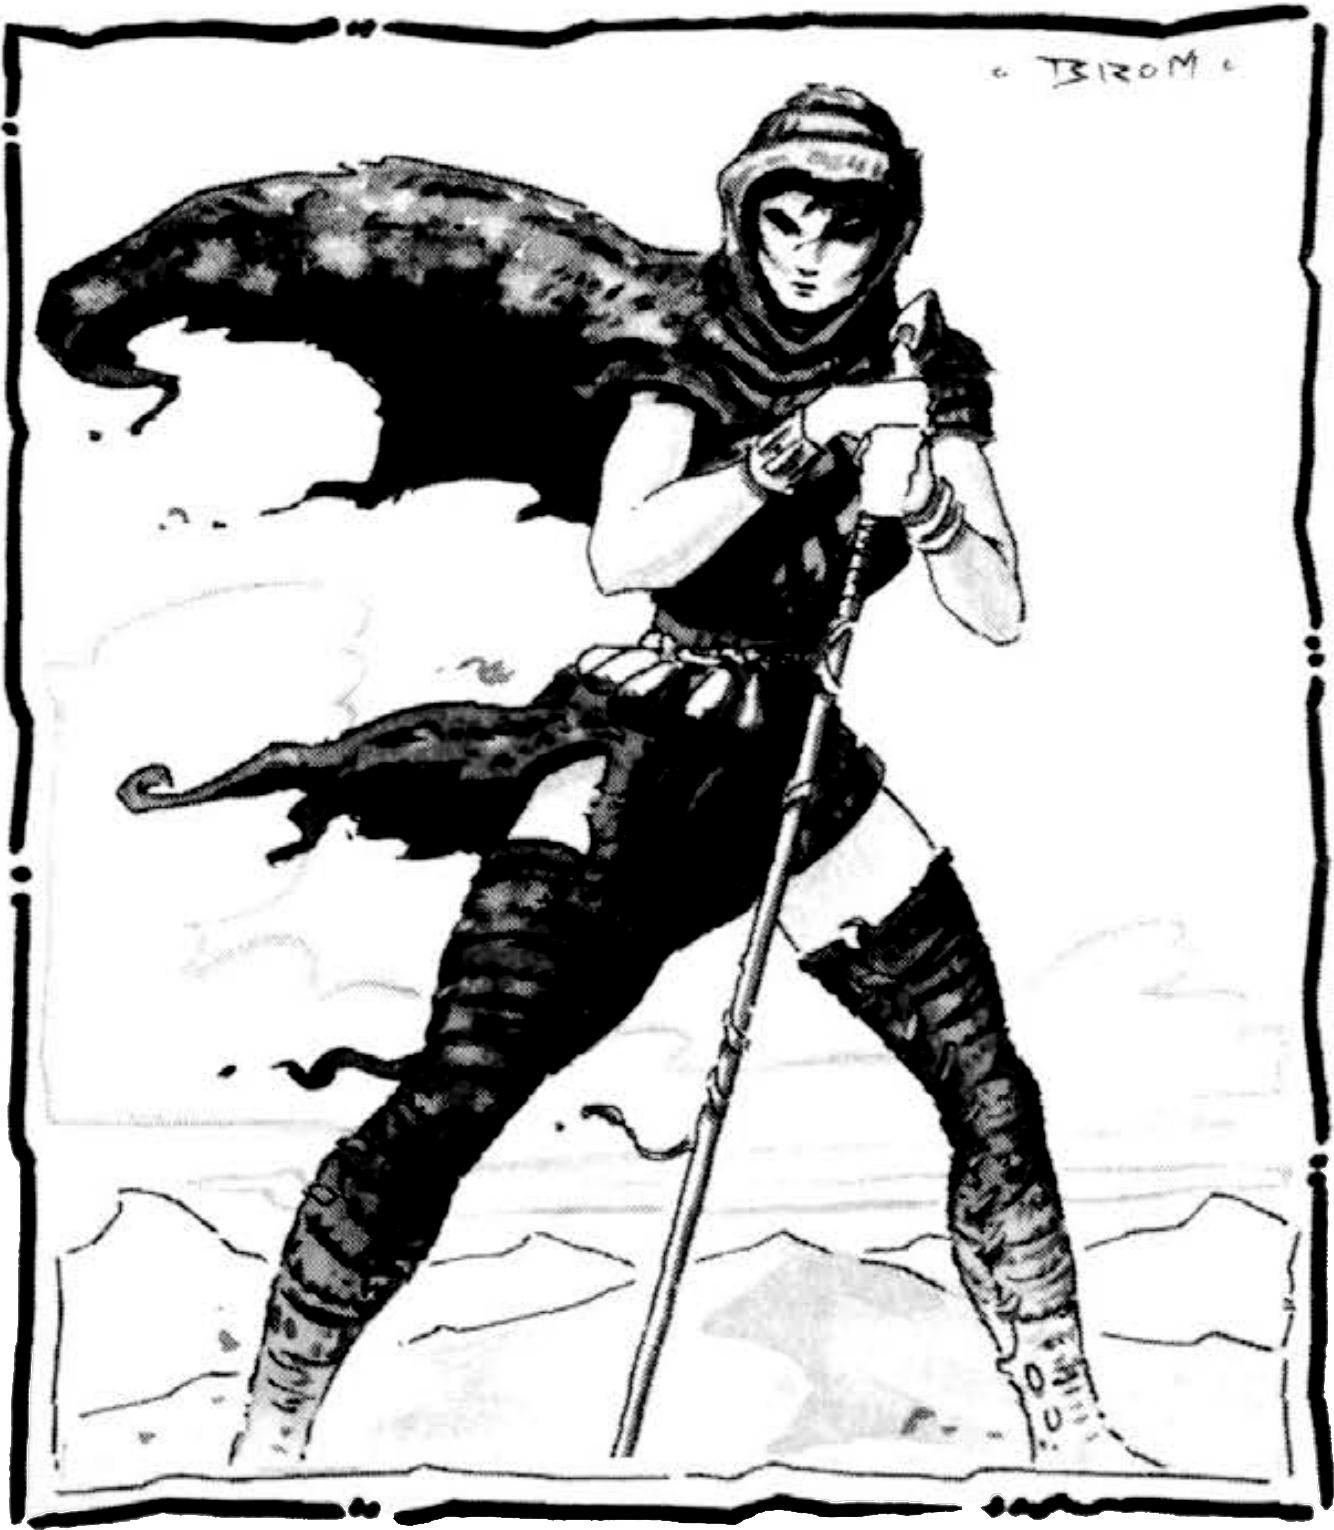
\includegraphics[width=\columnwidth]{images/halfelf-1.png}
\end{figure}
Unlike the parents of muls, elves and humans are often attracted to each other. Half-elves are typically the unwanted product of a casual interracial encounter.

\textbf{Personality:} Half-elves are notorious loners. Many Athasians believe that half-elves combine the worst traits of both races, but the most difficult aspect of half-elves---their lack of self-confidence comes not from their mixed origins but rather from a life of rejection from both parent races. Half-elves try in vain to gain the respect of humans or elves.

\textbf{Physical Description:} Averaging over 1.8 meters tall, half-elves combine Elven dexterity with human resilience. Bulkier than elves, most half-elves find it easier to pass themselves off as full humans than as full elves, but all have some features that hint at their Elven heritage.

\textbf{Relations:} Humans distrust the half-elf's Elven nature, while elves have no use for their mixed-blood children; Elven traditions demand that such children be left behind. Human society gives half-elves have a better chance of survival, but even less kindness. Half-elves sometimes find friendship among muls or even Thri-kreen. Half-elves will cooperate with companions when necessary, but find it difficult to rely on anyone. Many half-elves also turn to the animal world for company, training creatures to be servants and friends. Ironically, the survival skills and animal affinity that half-elves developed to cope with isolation make them valuable beast handlers in human society.

\textbf{Alignment:} Lawful and neutral half-elves labor for acceptance from a parent race, while chaotic ones have given up on acceptance, electing instead to reject the society that has rejected them.

\textbf{Half-Elven Lands:} Despite their unique nature, half-elves don't form communities. The few half-elves that settle down tend to live among humans who, unlike elves, at least find a use for them.

\textbf{Magic:} Half-elves often take up arcane studies, because it is a solitary calling.

\textbf{Psionics:} Mastery of the Way often provides the independence and self-knowledge that half-elves seek, and membership in a psionic academy can provide the half-elf with acceptance.

\textbf{Religion:} Because of their alienation from society and their affinity with animals, half-elves make excellent druids. Some half-elves turn their resentment of society into a profession and become sullen, bullying templars. As clerics, they are drawn to water's healing influence.

\textbf{Language:} Half-elves all speak the Common tongue. A few half-elves pick up the Elven language.

\textbf{Names:} Half-elves nearly always have human names. Unable to run as elves, they never receive Elven given names, or acceptance in an Elven tribe that they could use as surname.

\textbf{Adventurers:} In a party, half-elves often seem detached and aloof.

\subsection{Half-Elf Society}
Unlike other races, half-elves do not consider themselves a separate race, and, with very few exceptions, do not try to form half-Elven communities. A half-elf's life is typically harder than either a human's or an elf's. It is difficult for half-elves to find acceptance within either Elven or human society. Elves have not tolerance for those of mixed heritage, while humans do not trust their Elfish side. On the whole, humans are far more tolerant of half-elves than elves, who often refuse to allow such children into their tribes, and are likely to cast the half-elf's mother from the tribe as well.

Most half-elves consider themselves outsiders to all society and tend to wander throughout their entire lives, going through life as an outsider and loner. Half-elves are forced to develop a high level of self-reliance. Most half-elves take great pride in their self-reliance, but this pride often makes half-elves seem aloof to others. For many half-elves the detachment is a defensive mechanism to deal with a desire for acceptance from either human or Elven society that will likely never come. Some half-elves turn to the animal world for company, training creatures to be servants and friends.

\subsection{Roleplaying Suggestions}
Desperate for the approval of either elves or humans, you are even more desperate to appear independent and self-reliant, to cover your desire for approval. As a result, you tend towards a feisty, insecure, sullen self-reliance, refusing favors. You take every opportunity to show off your skills in front of elves and humans, but if an elf or a human were to actually praise you, you would probably react awkwardly or suspiciously. From your childhood, your closest friendships have been with animals. Other half-elves do not interest you. As time goes by and you learn from experience, you will find that you can also get along with other races neither human nor Elven: dwarves, pterran, muls, even thri-kreen. You don't feel the terrible need for their approval, and yet they give it more readily.

\subsection{Half-Elf Racial Traits}
\begin{itemize*}
    \item +2 Dexterity, $-2$ Charisma: Half-elves are limber like their Elven parents, but their upbringing leaves them with a poor sense of self, and affects their relations with others.
    \item Humanoid (elf): Half-elves are humanoid creatures with the elf subtype.
    \item Medium: As Medium creatures, half-elves have no bonuses or penalties due to size.
    \item Half-elf base land speed is 9 meters.
    \item Low-Light Vision: A half-elf can see twice as far as a human in starlight, moonlight, torchlight, and similar conditions of poor illumination. She retains the ability to distinguish color and detail under these conditions..
    \item Half-elves gain a +2 racial bonus to \skill{Disguise} checks when impersonating elves or humans.
    \item +1 racial bonus on \skill{Listen}, \skill{Search} and \skill{Spot} checks. Half-elves have keen senses, but not as keen as those of an elf.
    \item +2 racial bonus on all \skill{Survival} and \skill{Handle Animal} checks. Half-elves spend a lot of time in the wilds of the tablelands.
    \item Elven Blood: For all effects related to race, a half-elf is considered an elf. Half-elves, for example, are just as vulnerable to effects that affect elves as their elf ancestors are, and they can use magic items that are only usable by elves.
    \item Automatic Languages: Common and Elven. Bonus Languages: Any.
    \item Favored Class: Any. When determining whether a multiclass half-elf takes an experience point penalty, his highest-level class does not count when determining whether he takes an experience point for multiclassing.
\end{itemize*}
\section{Half-Giants}
\Quote{Mind of a child, strength of three grown men. I've seen a half-giant tear the walls out of a building because he wanted a better look at the tattoos on a mul inside.}{Daro, human trader}

Legend has it that in ages past, a sorcerer-queen used wizardry to beget a union of giant and human in order to create a race of powerful slaves. Whatever the truth of this legend, the half-giant race has increased in number and is now fairly common especially in human controlled lands near the shore of the Sea of Silt. Half-giants gain great strength, but dull wits, from their giant heritage, and are nearly as agile as their human forbearers.

\begin{figure}[t!]
\centering
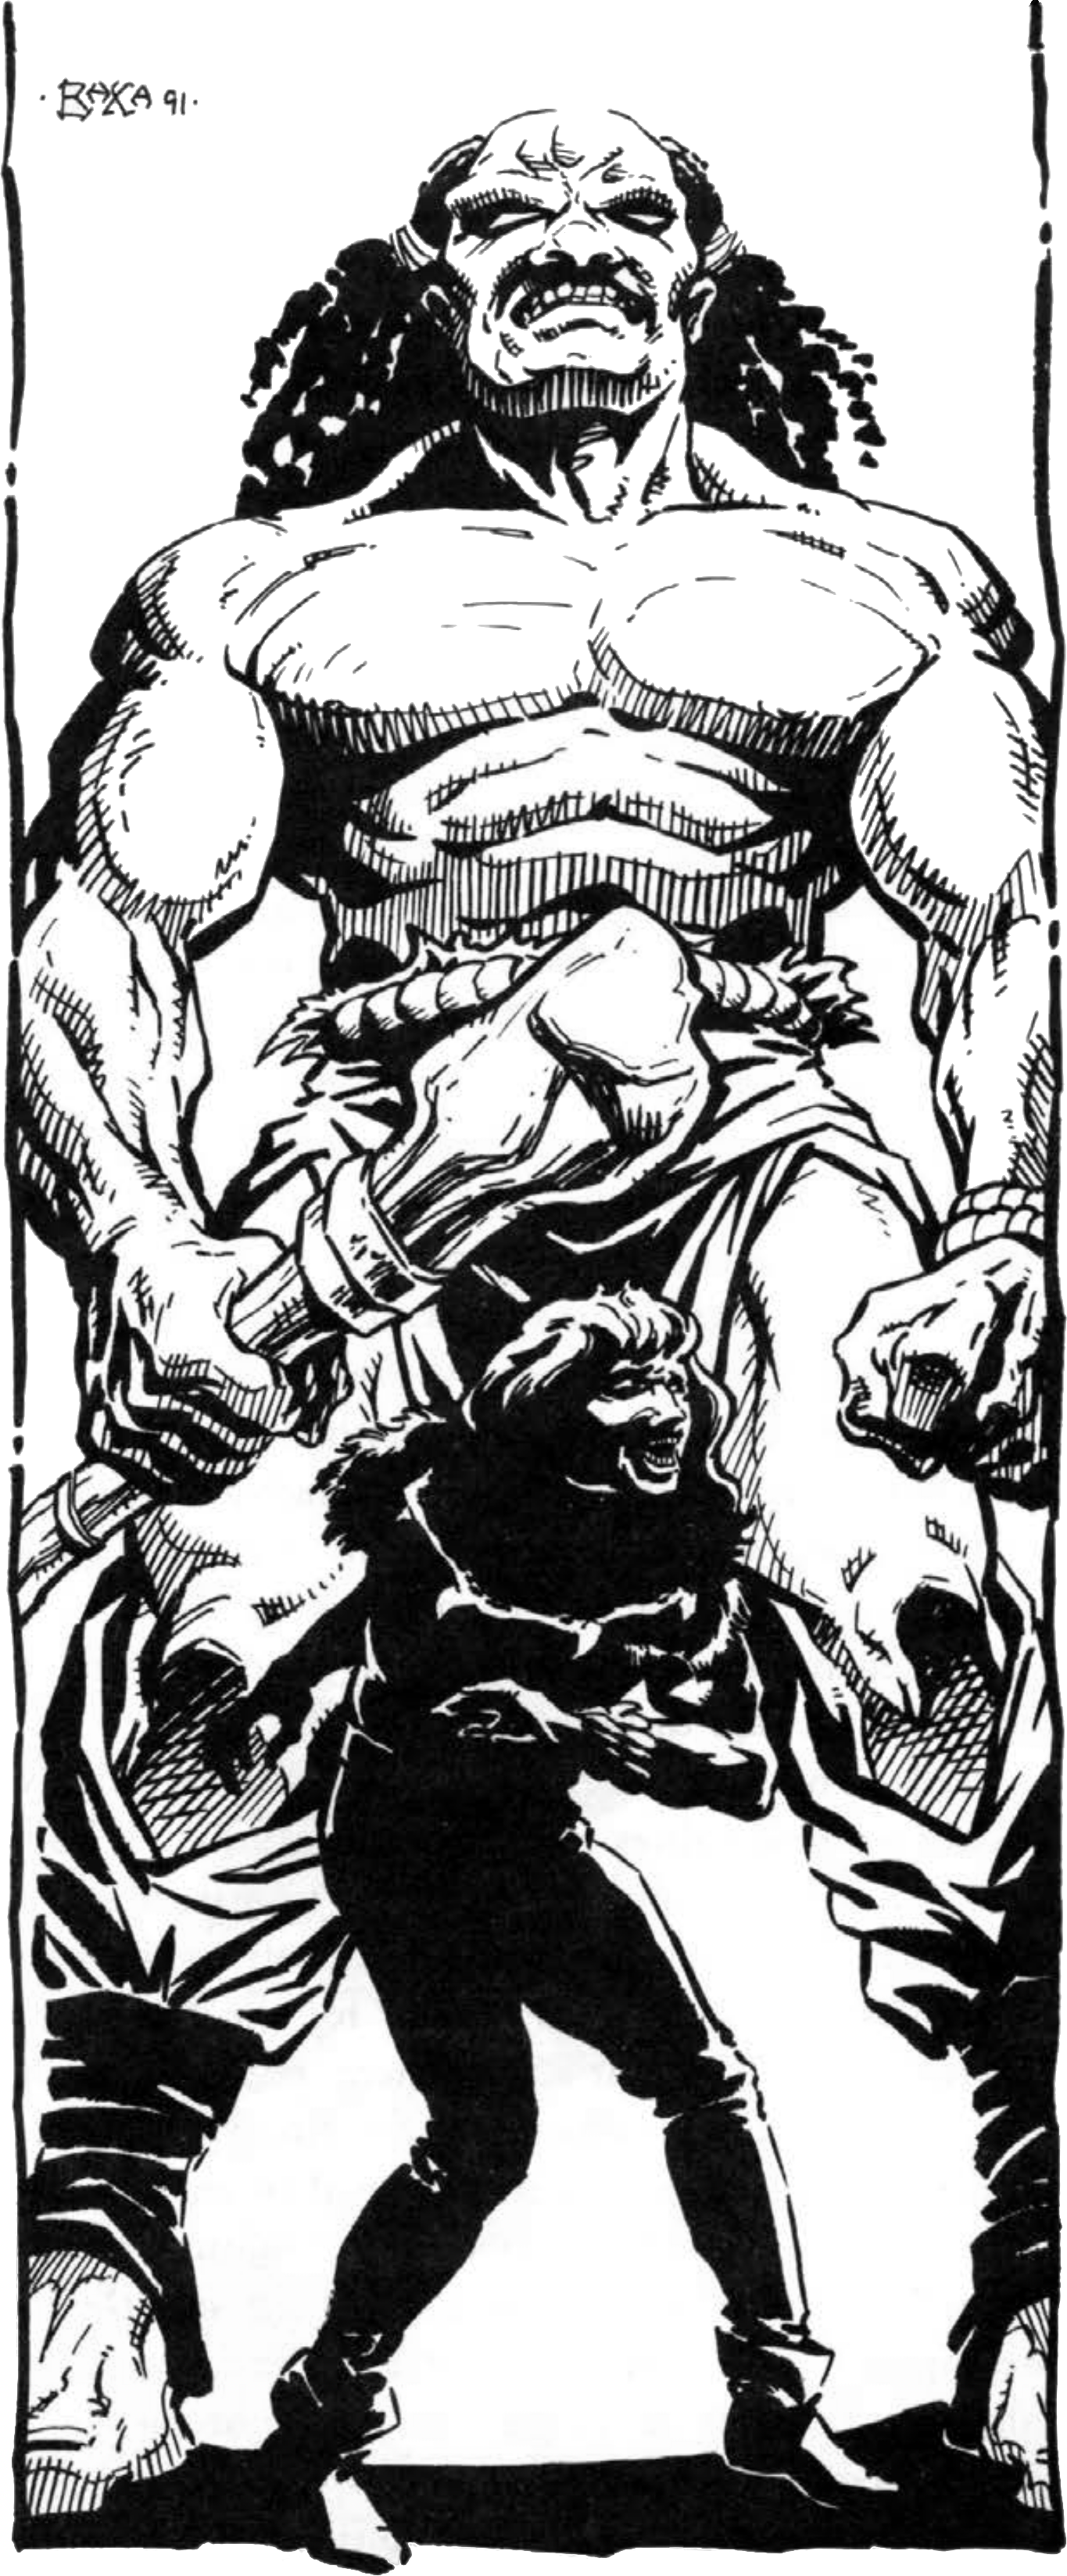
\includegraphics[width=\columnwidth]{images/halfgiant-1.png}
\WOTC
\end{figure}

\textbf{Personality:} Because of their artificial origins, there is no half-giant culture, tradition or homeland. Half-giants readily imitate the customs and cultures of their neighbors. Half-giants often display curiosity, a willingness to learn, and a general tendency towards kindness.

\textbf{Physical Description:} Physically, the half-giant is enormous, standing about 3.5 meters tall and weighing around 600 kg. Half-giants have thick hair, which is often kept braided (especially among females) or in a single tail that hangs behind the head and down the back. They dress in garb suitable to their occupation or environment. Half-giants mature at about 24 years of age and can live about 170 years.

\textbf{Relations:} The most powerful warriors on Athas, half-giants seem content to dwell in humanity's shadow. Half-giants tend to be friendly and eager to please, adopting the lifestyles, skills, and values of those they admire. A half-giant character who encounters a new situation looks around him to see what other people are doing. For example, a half-giant character that happens upon a Dwarven stone quarry may watch the dwarves, and then start quarrying stone himself. If he can make a living at it, he will continue to quarry stone just like his neighbor dwarves do; otherwise he will move on to something else.

\textbf{Alignment:} Half-giants can switch attitudes very quickly, taking on new values to fit new situations. A half-giant whose peaceful farming life is disrupted by marauders may soon adopt the morals of the renegades who sacked his village. A half-giant's nature is to switch his alignment aspect to imitate or otherwise react to a significant change around him.

\textbf{Half-Giant Lands:} Half-giants are most often found in the city-states, serving as gladiators, laborers, soldiers, and guards. A few half-giants collect into wilderness communities, often adopting the culture and customs of neighboring beings. The rare half-giant community often attaches itself to a charismatic or successful leader (not necessarily a half-giant) who demonstrates the tendencies they admire.

\textbf{Magic:} If a half-giant's companions accept wizardry, then the half-giant will also accept it. If a half-giant's companions hate wizardry, then the half-giant will be as eager as anyone to join in stoning a wizard. Among sophisticated companions who accept preserving magic but despise defiling magic, all but the brightest half-giants are likely to become confused, looking to their companions to see how they should react.

\textbf{Psionics:} While a single-classed half-giant psion is very rare, some half-giants take the path of the psychic warrior, becoming killing machines that can take apart a mekillot barehanded.

\textbf{Religion:} Half-giants do not display any affinity for the worship of one element over another.

\textbf{Language:} All half-giants speak the Common speech of slaves. Whatever tongue she speaks, the half-giant's voice is pitched so low as to occasionally be difficult to understand.

\textbf{Names:} Enslaved half-giants often have human names, and because of this they vary greatly. Free half-giants are likely to borrow the naming conventions of the race or people they are imitating at the time their child is born.

\textbf{Adventurers:} Half-giants are usually led to adventure by interesting companions of other races.

\subsection{Half-Giant Society}
A relatively young race, half-giants possess very little cultural identify of their own. Instead they adopt the customs and beliefs of those other cultures in which they live. Because of this, half-giants routinely change their alignment to match those around them who most influence them.
Half-giants can be found from one end of the Tablelands to the other, and often congregate in or near other population centers, absorbing the culture. Rarely do half-giants form communities of their own.

Unlike some other bastard races, half-giants can reproduce. A single off-spring is produced from half-giant unions after almost a year of pregnancy.

Though omnivorous, half-giants are tremendous consumers of water and food. They require twice the amount of food and water than humans. Clothing and equipment need twice the material to construct to fit a half-giant, leading to higher prices for half-giants.

Half-giants tend to damage objects and buildings around them through accidents of size alone. Some considerate half-giants camp outside city walls to avoid causing too much damage, but the draw of a city's culture and the below average intellect of most half-giants limits the number of half-giants who do so.

\subsection{Roleplaying Suggestions}
Always remember how much bigger and heavier you are than everyone else. Take advantage of your height in combat, but remember the disadvantages. Between your size and your lesser wits (even if you are a relatively intelligent half-giant people will assume you to be dull), you find yourself an object of comic relief. You are used to being teased and will endure more witty remarks than most people, but when you have been pushed too far your personality can suddenly shift, and you can unleash astonishing violence on your tormentors and any who stand in your way. Less frequently, these shifts can happen to you without provocation you just wake up with a different ethos and altered disposition.

Remember you are influenced by powerful personalities, and can shift your personality and ethics. You tend to imitate the tactics, clothes and demeanor of your ``little master.''
\subsection{Half-Giant Racial Traits}
\begin{itemize*}
    \item +8 Strength, +4 Constitution, $-2$ Dexterity, $-4$ Intelligence, $-4$ Wisdom, $-4$ Charisma: Half-giants are renowned for their great strength and dull wits.
    \item Large: As a Large creature, a half-giant takes a $-1$ penalty to Armor Class, a $-1$ penalty on attack rolls, and a $-4$ penalty on \skill{Hide} checks. She gains a +4 size bonus on grapple checks, and her lifting and carrying limits are double those of Medium characters, but she uses bigger weapons than humans use.
    \item Half-giants occupy a space of 3 meters and have a reach of 3 meters.
    \item Giant: Half-giants are creatures with the giant type.
    \item Half-giant base land speed is 12 meters.
    \item Darkvision: Half-giants can see in the dark out to 18 meters. Darkvision is black and white only, but it is otherwise like normal sight, and half-giants can function just fine with no light at all.
    \item Natural Armor: Half-giants have a +2 natural armor bonus to AC.
    \item Axis Alignment: One aspect of the half-giant's alignment must be fixed, and chosen during character creation. The other half must be chosen when they awake each morning. They are only bound to that alignment until they sleep again. For example, a half-giant may have a fixed lawful alignment. Every morning, he must choose to be lawful good, lawful neutral or lawful evil. This alignment change is not mandatory.
    \item Half-giants consume double the amount of food and water humans do.
    \item Favored Class: Barbarian. A multiclass half-giant's barbarian class does not count when determining whether he takes an experience point for multiclassing.
    \item Automatic Languages: Common. Bonus Languages: Dwarven, Gith, Giant. Half-giants will often pick up a race's tongue if imitating them long enough.
    \item Level Adjustment: +2. Half-giants are more powerful than the other races of the Tablelands and gain levels accordingly.
\end{itemize*}
\begin{figure*}[b!]
\centering
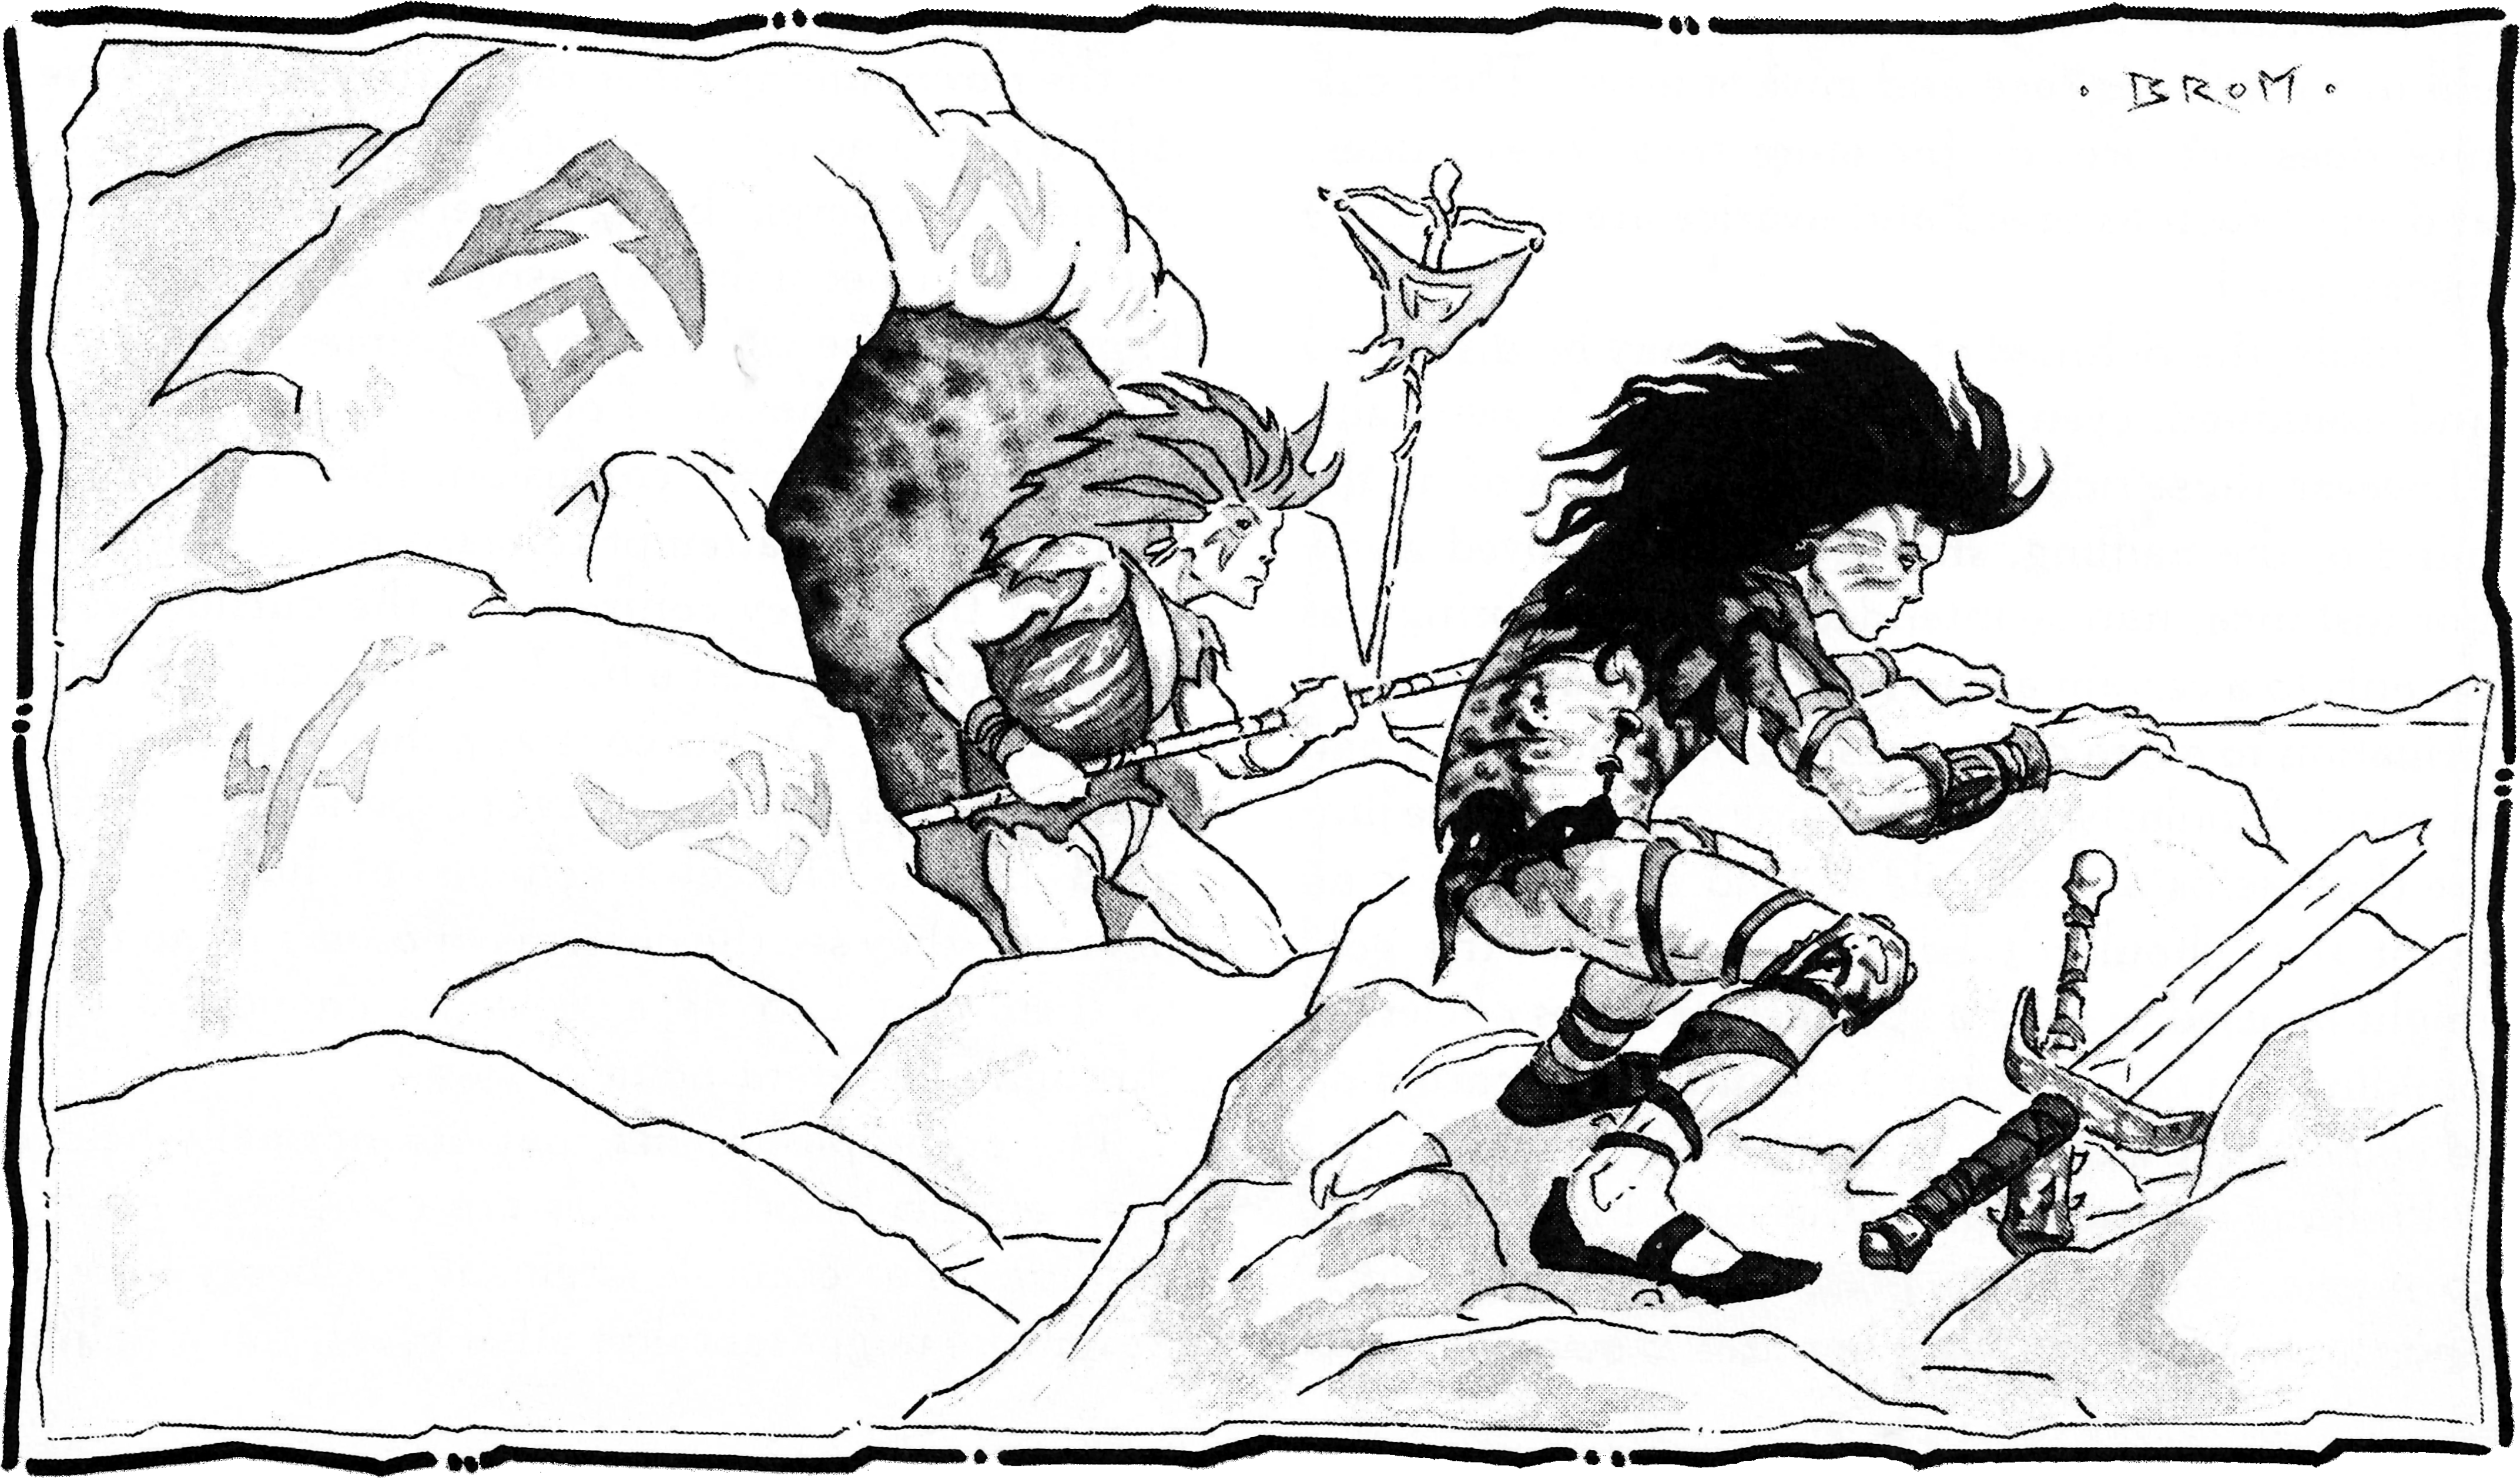
\includegraphics[width=\textwidth]{images/halfling-2.png}
\WOTC
\end{figure*}

\section{Halflings}
\Quote{Be wary of the forest ridge. The halflings who live there would as soon eat you alive as look at you. Chances are you won't even notice them until you've become the main course.}{Mo'rune, half-Elven ranger}

Halflings are masters of the jungles of the Ringing Mountains. They are small, quick and agile creatures steeped in an ancient and rich culture that goes back far into Athas' past. Although they are not common in the Tablelands, some halflings leave their homes in the forests to adventure under the{\tableheader Dark Sun}. As carnivores, halflings prefer to eat flesh raw.

\textbf{Personality:} Halflings have difficulty understanding others' customs or points of view, but curiosity helps some halflings overcome their xenophobia. Little concerned with material wealth, halflings are more concerned with how their actions will affect other halflings.

\textbf{Physical Description:} Halflings are small creatures, standing only about 1 meter tall and weighing 25 to 30 kilograms. Rarely affected by age, halfling faces are often mistaken for the faces of human children. They dress in loincloths, sometimes with a shirt or vest, and paint their skins with bright reds and greens. Forest halflings rarely tend to their hair, and some let it grow to great lengths, though it can be unkempt and dirty. They live to be about 120 years old.

\textbf{Relations:} Halfling's culture dominates their relations with others. They relate very well to each other, since they all have the same cultural traits and are able to understand each other. Halflings of different tribes still share a tradition of song, art and poetry, which serves as a basis of communication. Creatures that do not know these cultural expressions are often at a loss to understand the halfling's expressions, analogies and allusions to well-known halfling stories. Halflings can easily become frustrated with such ``uncultured'' creatures. They abhor slavery and most halflings will starve themselves rather than accept slavery.

\textbf{Alignment:} Halflings tend towards law and evil. Uncomfortable with change, halflings tend to rely on intangible constants, such as racial identity, family, clan ties and personal honor. On the other hand, halflings have little respect for the laws of the big people.

\textbf{Halfling Lands:} Halflings villages are rare in the tablelands. Most halflings live in tribes or clans in the Forest Ridge, or in the Rohorind forest west of Kurn. Many dwell in treetop villages. Non-halflings typically only see these villages from within a halfling cooking pot.

\textbf{Magic:} Many halfling tribes reject arcane magic. Tribes that accept wizards tend to have preserver chieftains. Only renegade halfling tribes are ever known to harbor defilers.

\textbf{Psionics:} Many halflings become seers or nomads. In the forest ridge, many tribal halflings become multiclassed seer/rangers, and become some of the deadliest trackers on Athas.

\textbf{Religion:} Halflings' bond with nature extends into most aspects of their culture. A shaman or witch doctor, who also acts as a spiritual leader, often rules their clans. This leader is obeyed without question. Halfling fighters willingly sacrifice themselves to obey their leader.

\textbf{Language:} Halflings rarely teach others their language, but some individuals of the Tablelands have learned the wild speech. Halflings found in the Tablelands often learn to speak Common.

\textbf{Names:} Halflings tend to have only one given name.

\textbf{Male Names:} Basha, Cerk, Derlan, Drassu, Entrok, Kakzim, Lokee, Nok, Pauk, Plool, Sala, Tanuka, Ukos, Zol.

\textbf{Female Names:} Alansa, Anezka, Dokala, Grelzen, Horga, Jikx, Joura, Nasaha, Vensa.

\textbf{Adventurers:} Exploring the Tablelands gives curious halflings the opportunity to learn other customs. Although they may at first have difficulty in understanding the numerous practices of the races of the Tablelands, their natural curiosity enables them to learn and interact with others. Other halflings may be criminals, renegades or other tribal outcasts, venturing into the Tablelands to escape persecution by other halflings.

\subsection{Halfling Society}
Most halflings have a common outlook on life that results in considerable racial unity across tribal and regional ties. Rarely will one halfling draw the blood of another even during extreme disagreements. Only renegade halflings do not share this racial unity, and are cast out of their tribes because of it.

Halfling society is difficult for other races to understand, as such concepts as conquest and plundering have no place. The most important value in halfling society is the abilities of the inner self as it harmonizes with the environment and the rest of the halfling race.

Halflings are extremely conscious of their environment. They are sickened by the ruined landscape of the Tyr region and desperately try to avoid having similar devastation occur to their homelands in the Forest Ridge. Most halflings believe that care must be taken to understand and respect nature and what it means to all life on Athas.

Halfling culture is expressed richly through art and song. Story telling in which oral history is passed on to the next generation is an important part of each halfling community. Halflings rely on this shared culture to express abstract thoughts and complicated concepts. This causes problems and frustration when dealing with non-halflings. Typically halflings assume that whomever they are talking to have the same cultural background to draw upon, and find it difficult to compensate for a listener who is not intimately familiar with the halfling history and ``lacks culture.''

Generally open-minded, wandering halflings are curious about outside societies and will attempt to learn all they can about other cultures. Never, will they adopt aspects of those cultures as their own, believing halfling culture to be innately superior to all others. Nor do they seek to change others' culture or views.

While halflings are omnivorous, they vastly prefer meat. Their meat heavy diet means that halflings view all living creatures, both humanoid and animal, as more food than equals. At the same time, most halflings believe that other races have the same perception of them. As a result, halflings are rarely likely to trust another member of any other race.

\subsection{Roleplaying Suggestions}
Remember to consistently take your height into account. Roleplay the halfling culture described above: eating opponents, treating fellow halflings with trust and kindness, suspicion of big people, and general lack of interest in money.

\subsection{Halfling Racial Traits}
\begin{itemize*}
    \item $-4$ Strength, +4 Dexterity, +4 Wisdom, $-2$ Charisma: Halflings are quick and stealthy, but weaker than humans.
    \item Humanoid (halfling): Halflings are humanoid creatures with the halfling subtype.
    \item Small: As a Small creature, a halfling gains a +1 size bonus to Armor Class, a +1 size bonus on attack rolls, and a +4 size bonus on \skill{Hide} checks, but she uses smaller weapons than humans use, and her lifting and carrying limits are three-quarters of those of a Medium character.%Halflings gain a +1 size bonus to Armor Class and a +1 size bonus on all attack rolls.
    \item Halfling base land speed is 6 meters.
    % \item Halflings receive a $-2$ penalty to all \skill{Diplomacy} skill checks when dealing with other races.
    \item +4 racial bonus on \skill{Climb} and \skill{Jump} checks: Halflings are agile.
    \item +2 racial bonus on saving throws against spells and spell-like effects.
    \item +1 racial attack bonus with a thrown weapon: javelins and slings are common weapons in feral halfling society, and many halflings are taught to throw at an early age.
    \item Halflings get advantage on \skill{Listen} checks---they have keen ears. Their senses of smell and taste are equally keen; they get advantage to all Wisdom checks that assess smell or taste.
    \item Halfings consume half the amount of food and water humans do.
    \item Automatic Languages: Halfling. Bonus Languages: Common, Dwarven, Elven, Gith, Kreen, Rhul-thaun, Sylvan, and Yuan-ti.
    \item Favored Class: Druid, Ranger, or Rogue. A halfling must choose between druid, ranger, or rogue as favored class. This choice cannot be changed. A multiclass halfling's chosen class does not count when determining whether he takes an experience point for multiclassing.
    \item Level Adjustment: +1.
\end{itemize*}
\section{Muls}
\Quote{See, the trick is to break their will. Not too much, mind you. Nobody wants to watch a docile gladiator, and muls are too expensive to waste as labor slaves. But, you don't want them trying to escape every other day. Would you like to tell the arena crowd that their favorite champion will not be appearing in today's match because he died trying to escape your pens?}{Gaal, Urikite arena trainer}

Born from the unlikely parentage of dwarves and humans, muls combine the height and adaptable nature of humans with the musculature and resilience of dwarves. Muls enjoy traits that are uniquely their own, such as their robust metabolism and almost inexhaustible capacity for work. The hybrid has disadvantages in a few areas as well: sterility, and the social repercussions of being created for a life of slavery. Humans and dwarves are not typically attracted to each other. The only reason that muls are so common in the Tablelands is because of their value as laborers and gladiators: slave-sellers force-breed humans and dwarves for profit. While mul-breeding practices are exorbitantly lucrative, they are often lethal to both the mother and the baby. Conception is difficult and impractical, often taking months to achieve. Even once conceived, the mul takes a full twelve months to carry to term; fatalities during this period are high. As likely as not, anxious overseers cut muls from the dying bodies of their mothers.

\textbf{Personality:} All gladiators who perform well in the arenas receive some degree of pampered treatment, but muls receive more pampering than others. Some mul gladiators even come to see slavery as an acceptable part of their lives. However, those that acquire a taste of freedom will fight for it. Stoic and dull to pain, muls are not easily intimidated by the lash. Masters are loath to slay or maim a mul who tries repeatedly to escape, although those who help the mul's escape will be tormented in order to punish the mul without damaging valuable property. Once a mul escapes or earns his freedom, slavery remains a dominant part of his life. Most muls are heavily marked with tattoos that mark his ownership, history, capabilities and disciplinary measures. Even untattooed muls are marked as a potential windfall for slavers: it is clearly cheaper to ``retrieve'' a mul who slavers can claim had run away, than to start from scratch in the breeding pits.

\begin{figure}[t!]
\centering
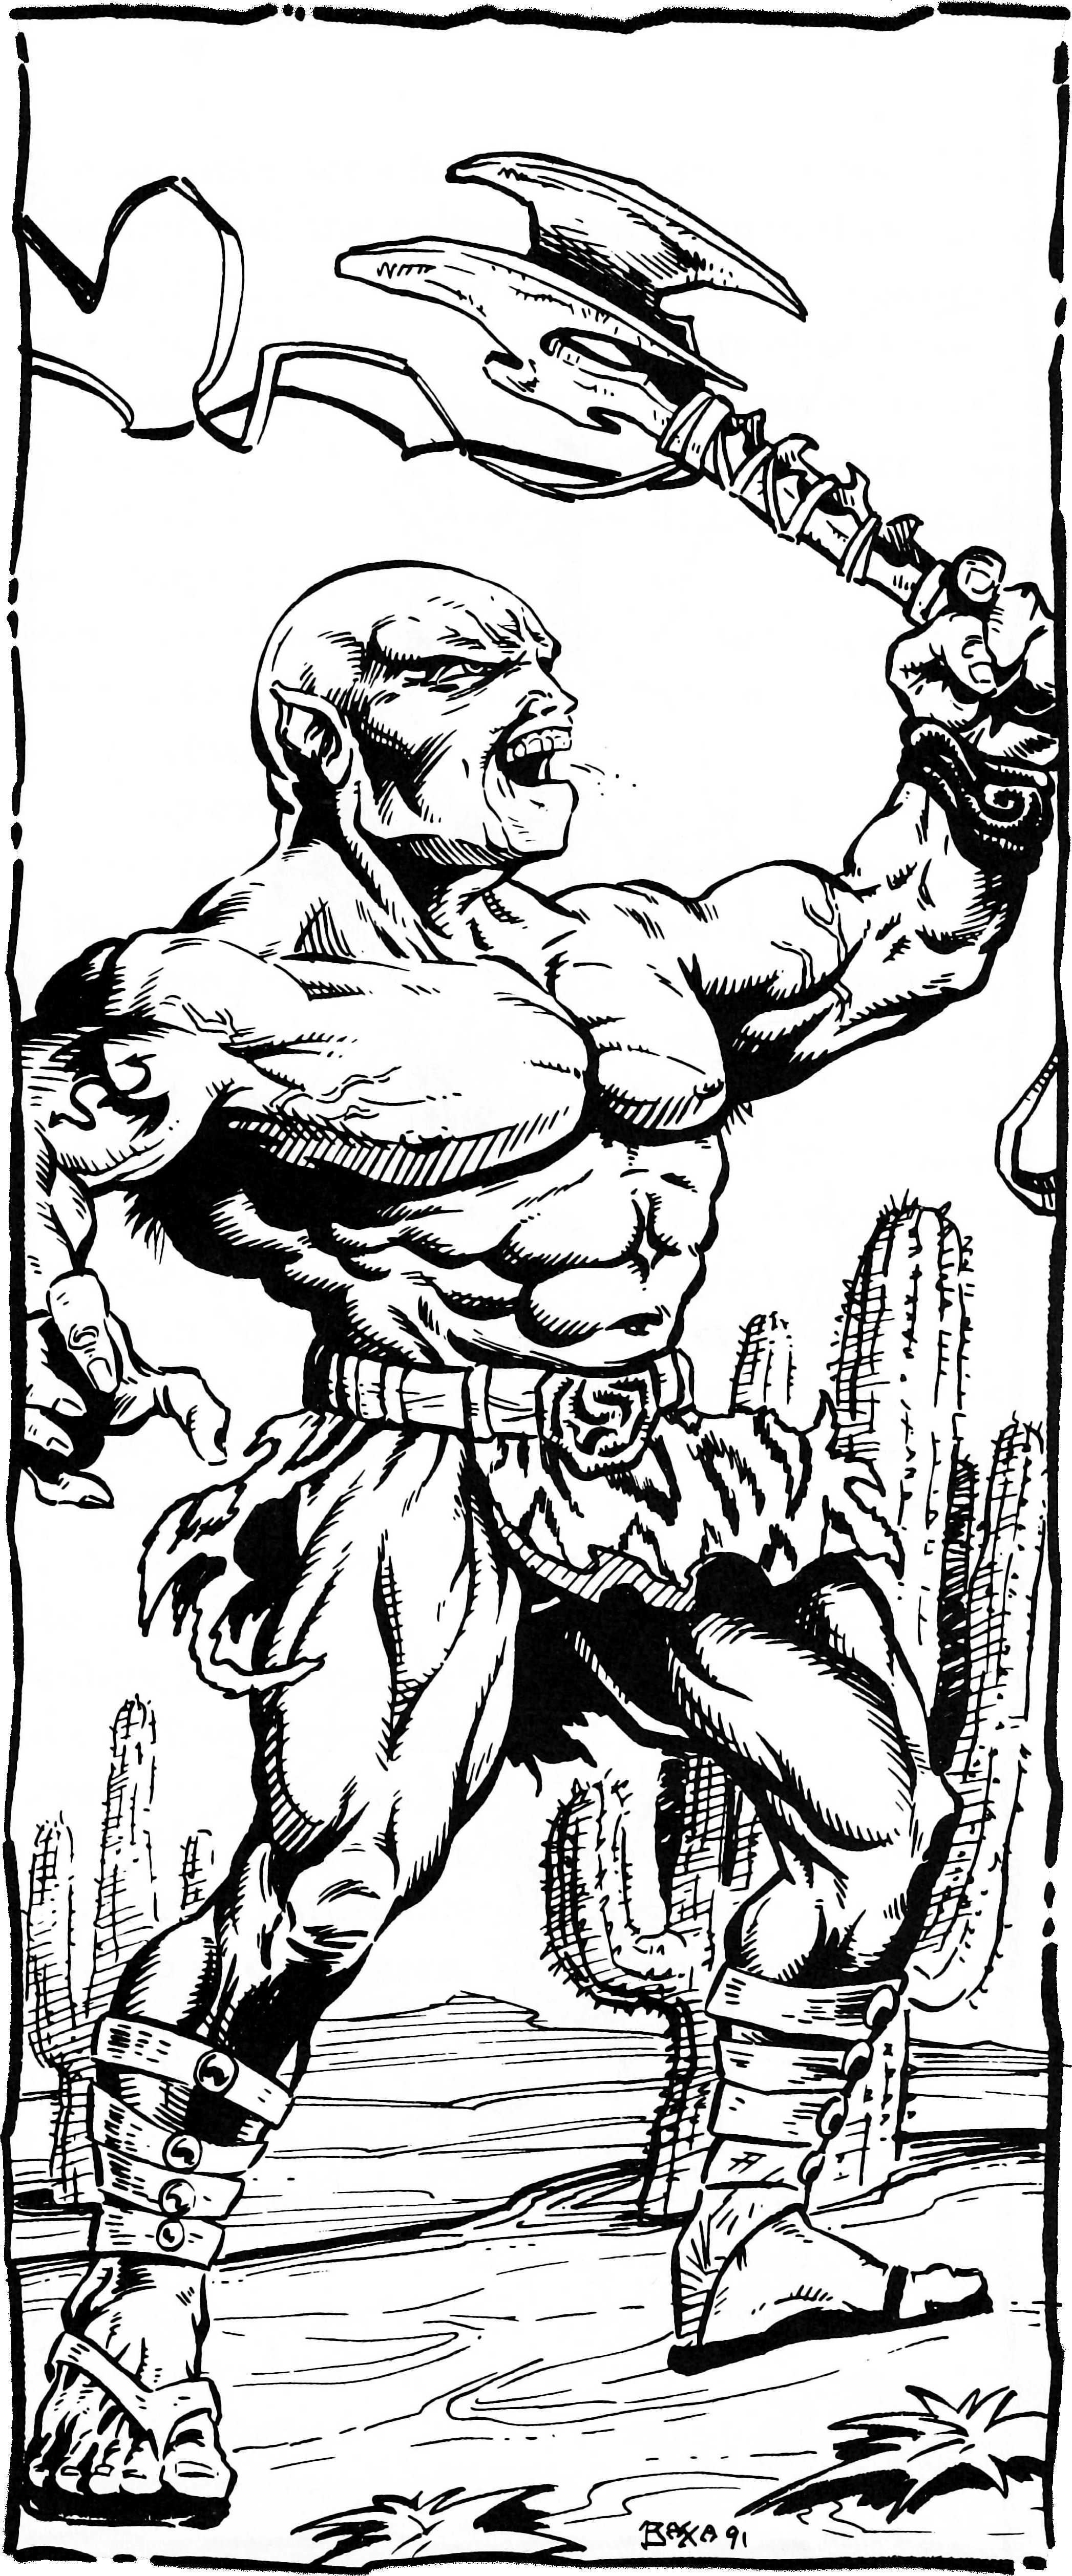
\includegraphics[width=\columnwidth]{images/mul-1.png}
\WOTC
\end{figure}

\textbf{Physical Description:} Second only to the half-giant, the mul is the strongest of the common humanoid races of the tablelands. Muls grow as high as 2.1 meters, weighing upwards of 125 kilograms, but carry almost no fat at all on their broad muscular frames. Universal mul characteristics include angular, almost protrusive eye ridges, and ears that point sharply backwards against the temples. Most muls have dark copper-colored skin and hairless bodies.

\textbf{Relations:} Most mul laborers master the conventions of slave life, figuring out through painful experience who can be trusted and who cannot. (Muls learn from their mistakes in the slave pits to a greater extent than other races not because they are cleverer, but because unlike slaves of other races they tend to survive their mistakes, while other slave races are less expensive and therefore disposable. Only the most foolish and disobedient mul would be killed. Most masters will sell a problem mul slave rather than kill him.) Their mastery of the rules of slave life and their boundless capacity for hard work allows them to gain favor with their masters and reputation among their fellow slaves.

\textbf{Alignment:} Muls tend towards neutrality with respect to good and evil, but run the gamut with respect to law or chaos. Many lawful muls adapt well to the indignities of slavery, playing the game for the comforts that they can win as valued slaves. A few ambitious lawful muls use the respect won from their fellow-slaves to organize rebellions and strike out for freedom. Chaotic muls, on the other hand, push their luck and their value as slaves to the breaking point, defying authority, holding little fear for the lash.

\textbf{Mul Lands:} As a collective group, muls have no lands to call their own. Occasionally, escaped muls band together as outlaws and fugitives, because of their common ex-slave backgrounds, and because their mul metabolism makes it easier for them to survive as fugitives while other races cannot keep up. Almost without exception, muls are born in the slave pits of the merchants and nobles of the city-states. Most are set to work as laborers, some as gladiators, and fewer yet as soldier-slaves. Very few earn their freedom, a greater number escape to freedom among the tribes of ex-slave that inhabit the wastes.

\textbf{Magic:} Muls dislike what they fear, and they fear wizards. They also resent that a wizard's power comes from without, with no seeming effort on the wizard's part, while the mul's power is born of pain and labor. Mul wizards are unheard of.

\textbf{Psionics:} Since most slave owners take steps to ensure that their property does not get schooled in the Way, it is rare for a mul to receive any formal training. Those that get this training tend to excel in psychometabolic powers.

\textbf{Religion:} Even if muls were to create a religion of their own, as sterile hybrids, they would have no posterity to pass it on to. Some cities accept muls as templars. Mul clerics tend to be drawn towards the strength of elemental earth.

\textbf{Language:} Muls speak the Common tongue of slaves, but those favored muls that stay in one city long enough before being sold to the next, sometimes pick up the city language. Because of their tireless metabolism, muls have the capacity to integrate with peoples that other races could not dream of living with, such as elves and Thri-kreen.

\textbf{Names:} Muls sold as laborers will have common slave names. Muls sold as gladiators will often be given more striking and exotic names. Draji names (such as Atlalak) are often popular for gladiators, because of the Draji reputation for violence. Masters who change their mul slaves' professions usually change their names as well, since it is considered bad form to have a gladiator with a farmer's name, and a dangerous incitement of slave rebellions to give a common laborer the name of a gladiator.

\textbf{Adventurers:} Player character muls are assumed to have already won their freedom. Most freed mul gladiators take advantage of their combat skills, working as soldiers or guards. Some turn to crime, adding rogue skills to their repertoire. A few muls follow other paths, such as psionics, templar orders or elemental priesthoods.

\subsection{Mul Society}
Muls have no racial history or a separate culture. They are sterile and cannot reproduce, preventing them from forming family groups and clans. The vast majority of muls are born in slavery, through breeding programs. Often the parents resent their roles in the breeding program and shun the child, leaving the mul to a lonely, hard existence. The taskmaster's whip takes the place of a family. For these reasons, many muls never seek friends or companionship, and often have rough personalities with tendencies towards violence.

The mul slave trade is very profitable, and thus the breeding programs continue. A slave trader can make as much on the sale of a mul as he could with a dozen humans. As slaves, a mul has his profession selected for him and is given extensive training as he grows.

Mul gladiators are often very successful, and win a lot of money for their owners. Highly successful gladiators are looked after by their owners, receiving a large retinue of other slaves to tend to their whims and needs. This has lead to the expression, ``pampered like a mul,'' being used often by the common folk.

Muls not trained as gladiators are often assigned to hard labor and other duties that can take advantage of the mul's hardy constitution and endurance.

\subsection{Roleplaying Suggestions}
Born to the slave pens, you never knew love or affection; the taskmaster's whip took the place of loving parents. As far as you have seen, all of life's problems that can be solved are solved by sheer brute force. You know to bow to force when you see it, especially the veiled force of wealth, power and privilege. The noble and templar may not look strong, but they can kill a man with a word. You tend towards gruffness. In the slave pits, you knew some muls that never sought friends or companionship, but lived in bitter, isolated servitude. You knew other muls who found friendship in an arena partner or co-worker. You are capable of affection, trust and friendship, but camaraderie is easier for you to understand and express - warriors slap each other on the shoulder after a victory, or give their lives for each other in battle. You don't think of that sort of event as ``friendship'' - it just happens.

\subsection{Mul Racial Traits}
\begin{itemize*}
    \item +4 Strength, +2 Constitution, $-2$ Intelligence, $-4$ Charisma: Combining the human height with the Dwarven musculature, muls end up stronger than either parent race, but their status as born-to-be slaves makes them insecure in their dealings with others.
    \item Humanoid (dwarf): Muls are humanoid creatures with the dwarf subtype.
    \item Medium: As Medium creatures, muls have no bonuses or penalties due to size.
    \item Mul base land speed is 9 meters.
    % \item Darkvision: Muls can see in the dark up to 9 meters. Darkvision is black and white only, but is otherwise like normal sight, and muls can function just fine with no light at all.
    \item Muls have +2 racial bonus on his damage rolls with light or thrown weapons (including unarmed strikes).
    \item Extended Activity: Muls require double the amount of time before making any check related to endurance.
    \begin{itemize*}
        \item Muls need to sleep every two days (but may choose to sleep every day);
        \item Muls can walk for 16 hours before beginning a forced march;
        \item Muls can hold their breath or run for a number of rounds equal to four times their Constitution score;
        \item Muls can go without food for six days;
        \item Muls can go without water for two days plus a number of hours equal to twice their Constitution score;
        \item Muls make Constitution checks every two hours of marching beyond 16 hours;
        \item Muls make Constitution checks every two rounds to continue holding their breath or running;
        \item Muls make Fortitude checks every two hours in a very hot (32 °C to 42 °C) or very cold ($-17$ °C to 4 °C) environments, every 20 minutes in severe heat (43 °C to 60 °C) or severe cold ($-28$ °C to $-18$ °C), and every 10 minutes in extreme heat \hskip10cm (61 °C to 82 °C), extreme cold ($-45$ °C to $-29$ °C), or worse environments;
        \item Muls make Constitution checks every two days after the first period without food;
        \item Muls make Constitution checks every two hours after the first period without water.
    \end{itemize*}
    % \item Tireless: Muls get a +4 racial bonus to checks for performing a physical action that extends over a period of time (running, swimming, holding breath, and so on). This bonus stacks with the \feat{Endurance} feat. This bonus may also be applied to savings throws against spells and magical effects that cause weakness, fatigue, exhaustion or enfeeblement.
    % \item Extended Activity: Muls may engage in up to 12 hours of hard labor or forced marching without suffering from the associated nonlethal damage and fatigue.
    \item Dwarven Blood: For all effects related to race, a mul is considered a dwarf. Muls, for example, are just as vulnerable to effects that affect dwarves as their dwarf ancestors are, and they can use magic items that are only usable by dwarves.
    % \item Nonlethal Damage Resistance 1/--. Muls are difficult to subdue, and do not notice minor bruises, scrapes, and other discomforts that pain creatures of other races.
    \item Favored Class: Fighter or Gladiator. A mul must choose between fighter or gladiator as favored class. This choice cannot be changed. A multiclass mul's chosen class does not count when determining whether he takes an experience point for multiclassing.
    \item Automatic Language: Common. Bonus Languages: Dwarven, Elven, Gith, and Giant.
    \item Level Adjustment: +1.
\end{itemize*}
% \section{Pterrans}
\Quote{The people of the Tablelands know nothing of life. They choose no Path for themselves, and consume everything until they are dead.}{Keltruch, pterran ranger}

\begin{figure}[b!]
\centering
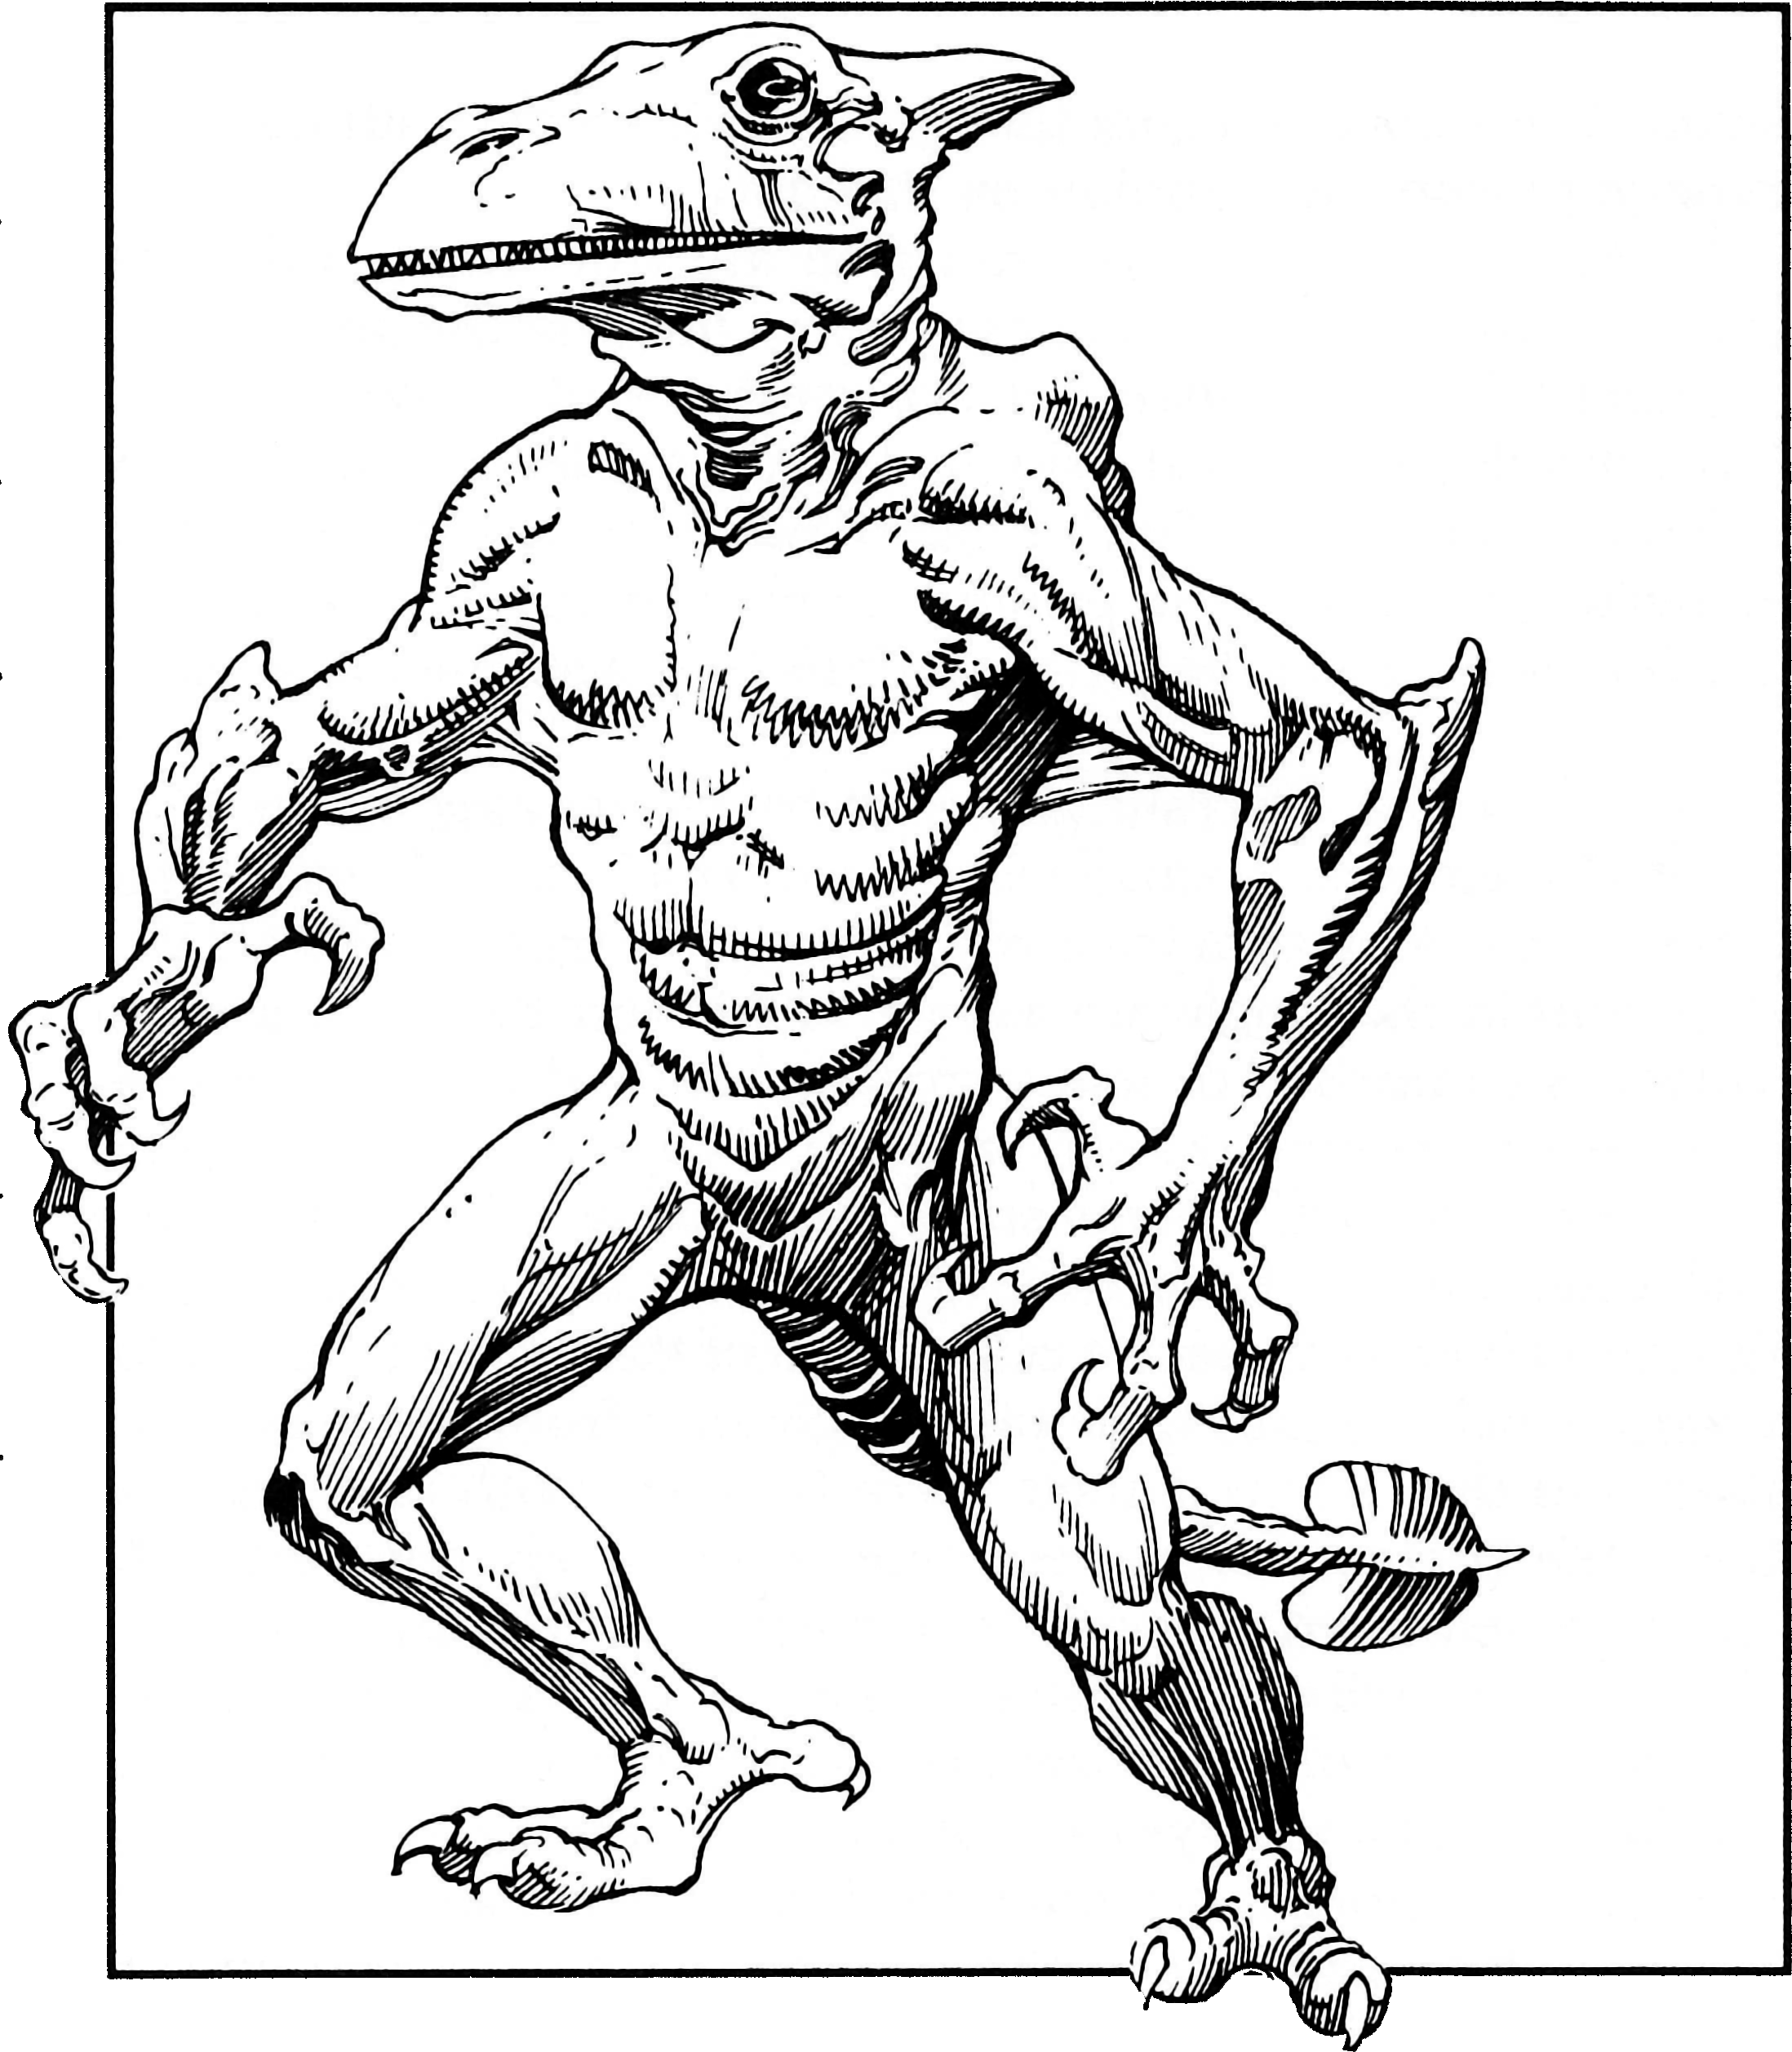
\includegraphics[width=\columnwidth]{images/pterran-1.png}
\end{figure}

Pterrans are rarely seen in the Tablelands. They live their lives in the Hinterlands, rarely leaving the safety of their villages. However, the recent earthquake and subsequent storms have brought disruption into the pterran's lives. More pterrans now venture outside their homes, and come to the Tyr region to seek trade and information.

\textbf{Personality:} Among strangers, pterrans seem like subdued, cautious beings, but once others earn a pterran's trust, they will find an individual that is open, friendly, inquisitive, and optimistic. In other respects, a pterran's personality is largely shaped by her chosen life path: Pterrans who choose the path of the warrior are less disturbed by the brutality of the Tablelands; they are constantly examining their surroundings and considering how the terrain where they are standing could be defended; they take greatest satisfaction from executing a combat strategy that results in victory without friendly casualties. Pterrans who choose the path of the druid are most interested in plants, animals, and the state of the land; they take greatest satisfaction when they eliminate a threat to nature. Pterrans that choose the path of the mind are most interested in befriending and understanding other individuals and societies; these telepaths take greatest satisfaction from intellectual accomplishments such as solving mysteries, exposing deception, resolving quarrels between individuals, and establishing trade routes between communities.

\textbf{Physical Description:} Pterrans are 1.5 to 1.9 meters tall reptiles with light brown scaly skin, sharp teeth, and a short tail. Pterrans wear little clothing, preferring belts and loincloths, or sashes. They walk upright, like humanoids, and have opposing thumbs and three-fingered, talon-clawed hands. Pterrans have two shoulder stumps, remnants of wings they possessed long ago, and a finlike growth juts out at the back of their heads. Pterrans weigh between 90 to 110 kilograms. There is no visible distinction between male and female pterrans.

\textbf{Relations:} Pterrans are new to the Tablelands, and unaccustomed to cultures and practices of the region. They have learned to not judge too quickly. Their faith in the Earth Mother means they undertake their adventure with open minds, but they will remain subdued and guarded around people they do not trust. A pterran's respect for the Earth Mother governs all his behavior. Creatures that openly destroy the land or show disrespect for the creatures of the wastes are regarded suspiciously. Pterrans understand the natural cycle of life and death, but have difficulty with some aspects of the city life, such as cramped living spaces, piled refuse, and the smells of unwashed humanoids.

\textbf{Alignment:} Pterrans tend towards lawful, well-structured lives, and most of them are good. Evil pterran adventurers are usually outcasts who have committed some horrible offense.

\textbf{Pterran Lands:} Most adventuring pterrans come from one of two villages in the Hinterlands, southwest of the Tyr regions: Pterran Vale and Lost Scale.

\textbf{Magic:} The wizard's use of the environment as a source of power conflicts with a pterran's religious beliefs. Pterrans will cautiously tolerate members of other races who practice preserving magic, if the difference is explained to them.

\textbf{Psionics:} Virtually all pterrans have a telepathic talent, and pterran psions are nearly universally telepaths. Telepathy is considered one of the honored pterran ``life paths.''

\textbf{Religion:} Pterrans worship the Earth Mother, a representation of the whole world of Athas. Their devotion to the Earth Mother is deeply rooted in all aspects of their culture, and it defines a pterran's behavior. All rituals and religious events are related to their worship of the Earth Mother. Religious events include festivals honoring hunts or protection from storms, with a priest presiding over the celebration. Most pterran priests are druids.

\textbf{Language:} Pterran speak Saurian with an accent that is difficult for other races to understand. The long appendage at the back of their head enables them to create sounds that no other race in the Tablelands can reproduce. The sounds are low, and resonate through the pterran's crest. Humanoid vocal chords cannot reproduce such sounds. Pterrans learn the Common tongue easily, but speak it with a slight, odd accent.

\textbf{Names:} Pterrans earn their first name just after they hatch, based on the weather and season of their hatching. After the pterran has decided upon a Life Path and has completed their apprenticeship, she receives title that becomes the first part of her name. This marks her transition into pterran society. There are a number of traditional names associated with each Life Path, but names do not always come from these ranks.

\textbf{Male Names:} Airson, Darksun, Earthsong, Suntail, Goldeye, Onesight, Terrorclaw.

\textbf{Female Names:} Cloudrider, Greenscale, Lifehearth, Rainkeeper, Spiritally, Watertender.

\textbf{Path Name:} Aandu, Caril, Dsar, Everin, Illik, Myril, Odten, Qwes, Pex, Ptellac, Ristu, Ssrui, Tilla, Xandu.

\textbf{Tribe or Village Names:} Pterran Vale, Lost Scale

\textbf{Adventurers:} Pterrans adventure because they believe the recent earthquake and disturbing events are signs from the Earth Mother that they should get more involved in the planet's affairs. They believe that these recent upheavals of nature are signs that the Earth Mother needs help, and this is a call the pterrans will gladly accept. As such, the most brave and adventurous of the pterrans have begun to establish contact with Tyr and some merchant houses, hoping to expand their contacts and information.

\subsection{Pterran Society}
Pterran society is based largely on ceremony and celebrations. An area is set aside in the center of each village for ceremonies. Pterrans revere the world of Athas as the Earth Mother, and believe themselves to be her favored children. Throughout the day, they engage in a number of ceremonies that give thanks to the Earth Mother. These are led by druids who play a very important role in pterran society.

A pterran village is a collection of many smaller family dwellings. Pterrans always bear young in pairs.

At age 15 every pterran chooses a ``life path.'' The three main life paths are the path of the warrior, the path of the druid and the path of the psionicist, though lesser life paths exist as well.

More pterrans follow the path of the warrior than any of the other paths, and become protectors of their villages as well as the tribe's weapon makers.

Pterrans that choose the path of the druid provide an important role in the daily ceremonies to the Earth Mother.

Fewer pterrans choose the path of the psionicist than the other two major paths, as psionics are viewed as outside of nature. Psionicists are viewed with suspicion by the rest of the tribe; however, they do provide valuable skills to the tribe and are often the tribe's negotiators when they meet outsiders.

Pterrans are omnivores. Much of their diet comes from hunting animals and raising crops. Kirre, id fiend, and flailer are all considered pterran delicacies.

\subsection{Roleplaying Suggestions}
Remember your character class is your ``life path.'' You think of yourself, and present yourself first and foremost as a druid, a warrior or a psion. Remember your daily celebrations and giving of thanks to the Earth Mother. You can usually find a reason to be grateful. Disrespect for the land angers you, since the whole land has withered under the disrespect of foolish humans and others. You celebrate with song and with dance. You have a good sense of humor but it does not extend to blasphemies such as defiling. In initial role-playing situations, you are unfamiliar with the customs and practices of the societies of the Tyr Region. However, you are not primitive by any definition of the word. You look upon differences with curiosity and a willingness to learn, as long as the custom doesn't harm the Earth Mother or her works.

\subsection{Pterran Racial Traits}
\begin{itemize*}
    \item $-2$ Dexterity, +2 Wisdom, +2 Charisma: Pterrans' strong confidence and keen instincts for others' motives make them keen diplomats, and when they take the path of the psion, powerful telepaths.
    \item Humanoid (psionic, reptilian): Pterrans are humanoid creatures with the psionic and reptilian subtypes.
    \item Medium: As Medium creatures, pterrans have no special bonuses or penalties due to size.
    \item Pterran base land speed is 9 meters.
    \item Poor Hearing: Pterrans have only slits for ears, and their hearing sense is diminished. Pterrans suffer a $-2$ penalty to Listen checks.
    \item Natural Weaponry: Pterrans can use their natural weapons instead of fighting with crafted weapons if they so choose. A pterran can rake with their primary claw attack for 1d3 of damage for each claw, and they bite for 1d4 points of damage as a secondary attack.
    \item Psi-Like Ability: At will---\psionic{missive}. All pterrans are gifted from the day they hatch with the ability to communicate telepathically, but only with their fellow reptiles. Manifester level is equal to \onehalf Hit Dice (minimum 1st).
    \item Weapon Familiarity: The following weapon is treated as martial rather than as an exotic weapon: thanak. This weapon is more common among pterrans than among other races.
    \item Automatic Languages: Saurian. Bonus Languages: Common, Dwarven, Elven, Halfling, Giant, Gith, Kreen, and Yuan-ti. Pterran know the languages of the few intelligent creatures that live in the Hinterlands.
    \item Life Path: A pterran's life path determines his favored class. Those following the Path of the Druid have druid as a favored class; the Path of the Mind gives psion as a favored class, while the Path of the Warrior gives ranger as a favored class. A Pterran chooses a life path upon coming of age, and the path cannot be changed once chosen at character creation time.
\end{itemize*}
\section{Thri-kreen}
\Quote{This one does not speak with the quivering soft shells that lay about all night. This one might eat you, but never speak.}{Tu'tochuk}

\Figure*{t}{images/thrikreen-1.png}

Thri-kreen are the strangest of the intelligent races of the Tablelands. These insectoid beings possess a mindset very different from any humanoid being encountered. They roam the wastes in packs, hunting for food day and night, since they require no sleep. Thri-kreen are quick and agile and make fearsome fighters, feared throughout the wastes.

\textbf{Personality:} Since thri-kreen (also known simply as the kreen) do not require sleep, they have difficulty understanding this need in the humanoid races. They have difficulty understanding this state of ``laziness'' in others. Other behaviors of humanoids seem unnecessarily complex. A keen's life is simple: hunt prey. Kreen live for the hunt, and own only what they can carry.

\textbf{Physical Description:} Mature thri-kreen stand about 2.1 meters tall, with a rough body length of 3.3 meters. Their four arms end in claws; their two legs are extremely powerful, capable of incredible leaps. However, kreen are unable to jump backwards. Their body is covered with a sandy-yellow chitin, a tough exoskeleton that grants the thri-kreen protection from blows. Their head is topped with two antennae, and their two eyes are compound and multifaceted. The kreen mouth consists of small pincers. Male and female thri-kreen are physically indistinguishable. Thri-kreen usually do not wear clothing, but wear some sort of harness to carry weapons and food. Many wear leg or armbands, or bracelets. Some attach rings on different places on their chitin, though this requires careful work by a skilled artisan.

\textbf{Relations:} The pack mentality dominates a keen's relation with others. Kreen hunt in packs, small groups that assemble together. Kreen will hunt prey in the same region for a while, but move on before their prey has been depleted. A kreen that joins a group of humanoids will often try to establish dominance in the group. This can be disconcerting to those unaware of the keen's behavior, since establishing dominance usually means making threatening gestures. Once the matter is settled, they will abide by the outcome. Thri-kreen view humanoids as sources of food, though they don't usually hunt them, only in dire need. Many kreen have a particularly fond taste for elves; as such, meetings between these two races are often tense. However, once part of a clutch, thri-kreen will never turn on their humanoid friends, even in the worst of situations.

\textbf{Alignment:} Most thri-kreen are lawful, since the pack mentality is ingrained in their beings. Kreen that deviate from this mentality are rare.

\textbf{Kreen Lands:} No thri-kreen settlements exist in the Tyr region; kreen encountered there are either small packs of kreen, or else adventuring with humanoids. To the north of the Tyr region, beyond the Jagged Cliffs, past the Misty Border, lies the Kreen Empire. This great nation of kreen rules the Crimson Savanna, forming great city-states that rival the humanoid city-states of the Tyr region.

\textbf{Magic:} Thri-kreen have no natural disposition towards magic, and a wizard's use of the environment as a source of power conflicts with a keen's beliefs. As well, the keen's lack of sleep and its instinctual need to hunt do not lend themselves well to magical study. Kreen wizards are extremely rare: no one has ever seen one in the Tablelands.

\textbf{Psionics:} Kreen view psionics as a natural part of their existence. Some packs rely on telepathy to communicate with each member and coordinate their hunting abilities. Many kreen also use psionic powers to augment their already formidable combat prowess. Psychometabolic powers are often used to boost speed, metabolism or strength to gain an advantage in combat. Most kreen (even non-adventurers) take the psychic warrior class, which kreen consider a natural part of growing up. Kreen do not need instruction to advance in the psychic warrior class---it comes to them as part of their ancestral memory.

\textbf{Religion:} Thri-kreen have no devotion to any god, but they hold nature and the elements in high regard. Ancestral memories guide them through their lives. Thri-kreen revere the Great One, a legendary kreen leader from the past.

\textbf{Language:} The Kreen language is very different from those of the other intelligent races. They have no lips or tongues, and so cannot make the same sounds humanoids make. Kreen language is made up of clicks, pops, or grinding noises.

\textbf{Names:} Kachka, Ka'Cha, Ka'Ka'Kyl, Klik-Chaka'da, Sa'Relka, T'Chai

\textbf{Adventurers:} Kreen adventure for different reasons. Most enjoy challenges presented by new prey. Some seek out the challenge of leading new clutches, new companions and observing the different ``hunting'' techniques of the dra (sentient meat-creatures such as humans).

\subsection{Thri-Kreen Society}
Thri-kreen hatch from eggs. All those who hatch at the same time form what is called a clutch. Thri-kreen gather in packs that roam the wastes. Each pack consists of several clutches that roam over an area that the pack considers theirs to hunt on. There are no permanent thri-kreen communities.

Clutches and packs are organized along strict order of dominance. The toughest member is leader; the second most powerful is second in command and so forth. A thri-kreen can challenge a superior for dominance initiating a contest. The contestants fight until one surrenders or dies. Afterwards, the matter is considered settled and there are no lingering resentments between victor and loser. The pack-mates take the view that the challenger was only acting to strength the pack.

Thri-kreen are obsessed with hunting. They are carnivores, but seldom hunt intelligent life for food. They do have a taste for elf, which gives them a bad reputation amongst Elven tribes. When not hunting, they craft weapons, teach their young, and craft sculptures.

The pack mentality is so ingrained in the culture that thri-kreen apply it to every situation. Thri-kreen feel compelled to be part of a clutch and will accept members of other races as clutch-mates.

\subsection{Roleplaying Suggestions}
You tend to rely on your natural attacks and special kreen weapons. Everything you kill is a potential dinner. You have a strong need for a party leader---obedience to this leader in the party is important to you. If you seem to be the most powerful and capable, then you will assume leadership; if someone challenges your authority then you will wish to test whether they are in fact stronger than you. It is not a question of vanity; you won't want to fight to the death, but merely to ascertain who is worthy to lead the party. You do not have the focus of a dwarf to complete a project, but you would give your life to protect your companions. If you did not trust and honor them as your own family, then you would not travel with them and work together with them. You do not understand the concept of sleep. It disturbs you that your dra companions lie unconscious for a third of their lifetimes. You own only what you can carry, caring little for money or other items that other races consider as treasure. Your philosophy of ownership sometimes leads you into conflict with presumptuous dra who think they can own buildings, land, and even whole herds of cattle!


% \Figure*{t}{images/adventurer-2.png}


\subsection{Thri-Kreen Racial Traits}
\begin{itemize*}
    \item +4 Dexterity, $-2$ Intelligence, +2 Wisdom, $-4$ Charisma: Thri-kreen are fast, but their alien mindset makes it difficult for them to relate to humanoids; furthermore, their ``clutch-mind'' instincts leave them with a poor sense of themselves as individuals.
    \item Monstrous Humanoid: Thri-kreen are not subject to spells or effects that affect humanoids only, such as \spell{charm person} or \spell{dominate person}.
    \item Medium: Thri-kreen receive no advantages or penalties due to size.
    \item Thri-kreen base land speed is 12 meters.
    \item Low-light Vision: Thri-kreen can see twice as far as a human in moonlight and similar conditions of poor illumination, retaining the ability to distinguish color and detail.
    \item Vestigial Antennae: Thri-kreen lessen miss chance from any type of concealment by 5\% (including total concealment or blindness). Thri-kreen have 15\% miss chance against foes with concealment, and 45\% miss chance against enemies with total concealment or when the thri-kreen is blinded.
    \item Sleep Immunity: Thri-kreen do not sleep, and are immune to sleep spells and similar effects. Thri-kreen spellcasters and manifesters still require 8 hours of rest before preparing spells or regaining power points.
    \item Water Efficient: Thri-kreen can go for one week on the amount of water a human needs in a day.
    \item Natural Armor: Thri-kreen have a +2 natural armor bonus to AC due to their naturally tough and resistant chitin.
    \item Multiple Limbs: Thri-kreen have four arms, and thus can take the \feat{Multiweapon Fighting} feat instead of the \feat{Two-Weapon Fighting} feat. Thri-kreen can also take the \feat{Multiattack} feat. (These are not bonus feats.)
    \item Natural Weapons: Thri-kreen may make bite and claw attacks as a full round action. Their primary claw attack does 1d4 points of damage for each of their four claws. Their secondary bite attack, deals 1d4 points of damage, and has a chance to poison. A thri-kreen can attack with a weapon (or multiple weapons) at its normal attack bonus, and make either a bite or claw attack as a secondary attack.
    \item Deflect Arrows: Thri-kreen gain the benefit of the \feat{Deflect Arrows} feat.
    \item Leap (Ex): When a thri-kreen reaches 3 Hit Dice, they become natural jumpers, gaining a +30 racial bonus to all \skill{Jump} checks.
    \item Poison (Ex): When a thri-kreen reaches 5 Hit Dice, their glands become able to deliver poison with a successful bite attack. Fortitude DC 11 + Con modifier. The initial and secondary damages are paralysis for 1d10 rounds.
    \item Weapon Familiarity: To thri-kreen, the chatkcha and gythka are treated as martial rather than exotic weapons. These weapons are more common among thri-kreen than among other races.
    \item Thri kreen have a +4 racial bonus on \skill{Hide} checks in sandy or arid areas.
    \item Alien Mind (Ex): A thri-kreen has difficulty understanding how the humanoid minds work. Whenever a thri-kreen targets a creature of another race with mind-affecting abilities, that creature gains +1 to its save against those powers.
    \item Automatic Languages: Kreen. Bonus Languages: Common, Dwarven, Elven, Entomic, Saurian, and Terran.
    \item Favored Class: Druid or Fighter. A thri-kreen must choose between druid or fighter as favored class. This choice cannot be changed. A multiclass thri-kreen's chosen class does not count when determining whether he takes an experience point for multiclassing.
    \item Level Adjustment: +1.
\end{itemize*}


\Figure*[\textwidth-5mm]{t}{images/tavern-2.png}
\section{Other Races}
% Athas is a place where members of different races are usually found in the same city-state, usually because they are going to be used in gladiatorial games as an exotic attraction, or to become slaves due to their physical might. Even though they are not usually concentrated on a specific area, these races are significant players in the Tablelands. It is only fitting then, that belgoi, gith, jozhals, ssurrans, tareks, taris, yuan-tis, and a variety of other creatures commonly viewed as monsters might appear as player characters in a {\tableheader Dark Sun} campaign. Cultural information about several monstrous races appears in \chapref{Life on Athas}.
Athas is a place where members of different races are usually found in the same city-state. Even though they are not usually concentrated on a specific area, these races are significant players in the Tablelands. It is only fitting then that a variety of other creatures commonly viewed as monsters might appear as player characters in a {\tableheader Dark Sun} campaign. Cultural information about several monstrous races appears in \chapref{Life on Athas}.
